\documentclass[12pt,a4paper,oneside]{report}

% ==============================================================================
% PACKAGE CONFIGURATIONS
% ==============================================================================
\usepackage[a4paper, top=2.5cm, bottom=2.5cm, left=3.0cm, right=2.0cm]{geometry}
\usepackage{setspace}
\onehalfspacing % 1.5 Line Spacing requirement

% Font: Times New Roman standard
\usepackage{mathptmx}
\usepackage[T1]{fontenc}
\usepackage[utf8]{inputenc}

% Mathematics packages
\usepackage{amsmath, amssymb, amsfonts}

% Tables & Formatting
\usepackage{booktabs}
\usepackage{tabularx}
\usepackage{multirow}
\usepackage{longtable}
\usepackage{array}
\usepackage{enumitem}

% Graphics & Colors
\usepackage{graphicx}
\usepackage{xcolor}
\usepackage{tikz}
\usetikzlibrary{shapes.geometric, arrows.meta, positioning, calc, backgrounds}

% Code Listings
\usepackage{listings}
\definecolor{codegreen}{rgb}{0,0.6,0}
\definecolor{codegray}{rgb}{0.5,0.5,0.5}
\definecolor{codepurple}{rgb}{0.58,0,0.82}
\definecolor{backcolour}{rgb}{0.97,0.97,0.98}

\lstdefinestyle{mystyle}{
    backgroundcolor=\color{backcolour},   
    commentstyle=\color{codegreen}\itshape,
    keywordstyle=\color{blue}\bfseries,
    numberstyle=\tiny\color{codegray},
    stringstyle=\color{codepurple},
    basicstyle=\ttfamily\footnotesize,
    breakatwhitespace=false,         
    breaklines=true,                 
    captionpos=b,                    
    keepspaces=true,                 
    numbers=left,                    
    numbersep=5pt,                  
    showspaces=false,                
    showstringspaces=false,
    showtabs=false,                  
    tabsize=2,
    frame=single,
    rulecolor=\color{codegray!30}
}
\lstset{style=mystyle}

% JSON listing support
\lstdefinelanguage{json}{
    basicstyle=\normalfont\ttfamily\footnotesize,
    numbers=left,
    numberstyle=\tiny\color{codegray},
    stepnumber=1,
    numbersep=8pt,
    showstringspaces=false,
    breaklines=true,
    frame=lines,
    backgroundcolor=\color{backcolour},
    literate=
     *{0}{{{\color{blue}0}}}{1}
      {1}{{{\color{blue}1}}}{1}
      {2}{{{\color{blue}2}}}{1}
      {3}{{{\color{blue}3}}}{1}
      {4}{{{\color{blue}4}}}{1}
      {5}{{{\color{blue}5}}}{1}
      {6}{{{\color{blue}6}}}{1}
      {7}{{{\color{blue}7}}}{1}
      {8}{{{\color{blue}8}}}{1}
      {9}{{{\color{blue}9}}}{1}
      {:}{{{\color{black}{: }}}}{1}
      {,}{{{\color{black}{, }}}}{1}
      {\{}{{{\color{black}{\{}}}}{1}
      {\}}{{{\color{black}{\}}}}}{1}
      {[}{{{\color{black}{[}}}}{1}
      {]}{{{\color{black}{]}}}}{1},
}

% Titlesec formatting: 16pt Chapter, 14pt Section, 12pt Subsection
\usepackage{titlesec}
\titleformat{\chapter}[display]
  {\normalfont\fontsize{16}{20}\bfseries}{\chaptertitlename\ \thechapter}{14pt}{\fontsize{16}{20}\bfseries}
\titleformat{\section}
  {\normalfont\fontsize{14}{18}\bfseries}{\thesection}{1em}{}
\titleformat{\subsection}
  {\normalfont\fontsize{12}{16}\bfseries}{\thesubsection}{1em}{}
\titlespacing*{\chapter}{0pt}{-20pt}{20pt}

% Header and Footer
\usepackage{fancyhdr}
\pagestyle{fancy}
\fancyhf{}
\fancyhead[L]{\small\nouppercase{\leftmark}}
\fancyhead[R]{\small B.Tech Major Project 1}
\fancyfoot[C]{\thepage}
\renewcommand{\headrulewidth}{0.5pt}
\renewcommand{\footrulewidth}{0.3pt}

% Hyperref
\usepackage[colorlinks=true, linkcolor=blue!80!black, citecolor=blue!80!black, urlcolor=blue!80!black]{hyperref}

% Table column helper types
\newcolumntype{Y}{>{\centering\arraybackslash}X}
\newcolumntype{L}{>{\raggedright\arraybackslash}X}

% ==============================================================================
% DOCUMENT CONTENT
% ==============================================================================
\begin{document}

% ------------------------------------------------------------------------------
% PRELIMINARY PAGES (ROMAN NUMERALS)
% ------------------------------------------------------------------------------
\pagenumbering{roman}
\thispagestyle{empty}

% 1. COVER PAGE / TITLE PAGE
\begin{center}
    \vspace*{0.3cm}
    {\fontsize{18}{22}\bfseries Multi-Agent Deep Reinforcement Learning for Adaptive Traffic Signal Control in Indian Corridors\par}
    
    \vspace{1.2cm}
    {\fontsize{14}{18}\bfseries MAJOR PROJECT - I\par}
    
    \vspace{1.2cm}
    {\fontsize{12}{16}\selectfont\textbf{Enrolment Numbers} -- 23104003, 23104005, 23104030\par}
    \vspace{0.4cm}
    {\fontsize{12}{16}\selectfont\textbf{Name of Students} -- Shivam Gupta, Tejas Srivastava, Anvit Singhal\par}
    
    \vspace{1.0cm}
    {\fontsize{12}{16}\selectfont\textbf{Name of Supervisor} -- Dr. Kapil Madan\par}
    
    \vfill
    \begin{figure}[h]
        \centering
        \begin{tikzpicture}
            \draw[thick, color=blue!70!black] (0,0) circle (1.2cm);
            \node[font=\bfseries\tiny, color=blue!80!black, align=center] at (0, 0.45) {JAYPEE INSTITUTE OF\\INFORMATION TECHNOLOGY};
            \node[font=\bfseries\large, color=orange!80!black] at (0, -0.05) {jiit};
            \node[font=\small, color=blue!90!black] at (0, -0.45) {विद्या तत्व ज्योतिसमः};
        \end{tikzpicture}
    \end{figure}
    \vspace{0.2cm}
    
    {\fontsize{12}{15}\selectfont\textbf{20th November 2026}\par}
    \vspace{0.5cm}
    {\fontsize{12}{15}\selectfont Submitted in partial fulfillment of the Degree Of\par}
    \vspace{0.2cm}
    {\fontsize{14}{17}\bfseries Bachelor of Technology\par}
    {\fontsize{12}{15}\selectfont In\par}
    {\fontsize{13}{16}\bfseries Information Technology\par}
    
    \vspace{0.8cm}
    {\fontsize{12}{15}\bfseries DEPARTMENT OF COMPUTER SCIENCE ENGINEERING \&\\INFORMATION TECHNOLOGY\par}
    \vspace{0.15cm}
    {\fontsize{13}{16}\bfseries JAYPEE INSTITUTE OF INFORMATION TECHNOLOGY,\\NOIDA\par}
\end{center}

\newpage
\thispagestyle{empty}

% 2. CERTIFICATE PAGE
\begin{center}
    {\fontsize{16}{20}\bfseries JAYPEE INSTITUTE OF INFORMATION TECHNOLOGY\\NOIDA\par}
    \vspace{0.3cm}
    {\fontsize{12}{15}\selectfont (Declared Deemed to be University u/s 3 of UGC Act 1956)\par}
    \vspace{1.5cm}
    {\fontsize{16}{20}\bfseries\underline{CERTIFICATE}\par}
\end{center}

\vspace{1.0cm}
\noindent This is to certify that the project report entitled \textbf{``Multi-Agent Deep Reinforcement Learning for Adaptive Traffic Signal Control in Indian Corridors,''} submitted by \textbf{Shivam Gupta (23104003), Tejas Srivastava (23104005), Anvit Singhal (23104030)} in partial fulfillment of the requirements for the award of the degree of \textbf{Bachelor of Technology in Information Technology} at \textbf{Jaypee Institute of Information Technology, Noida}, is an authentic record of the original work carried out by them under my supervision and guidance during the 7th Semester (Odd Semester, 2026).

\vspace{0.8cm}
\noindent To the best of my knowledge, the matter embodied in this report has not been submitted to any other University or Institute for the award of any degree or diploma.

\vspace{3.5cm}
\noindent
\begin{minipage}[t]{0.55\textwidth}
    \textbf{Dr. Kapil Madan}\\
    Project Supervisor\\
    Assistant Professor\\
    Department of CSE \& IT\\
    Jaypee Institute of Information Technology\\
    Noida, Uttar Pradesh
\end{minipage}

\newpage

% 3. DECLARATION OF ORIGINALITY
\begin{center}
    {\fontsize{16}{20}\bfseries\underline{CANDIDATE'S DECLARATION}\par}
\end{center}

\vspace{1.0cm}
\noindent We hereby declare that the work presented in this project report entitled \textbf{``Multi-Agent Deep Reinforcement Learning for Adaptive Traffic Signal Control in Indian Corridors,''} in partial fulfillment of the requirements for the award of the degree of \textbf{Bachelor of Technology in Information Technology}, submitted to the \textbf{Department of Computer Science Engineering \& Information Technology, Jaypee Institute of Information Technology, Noida}, is an authentic record of our own work carried out during the period from July 2026 to November 2026 under the supervision of \textbf{Dr. Kapil Madan}.

\vspace{0.8cm}
\noindent We further declare that we have not submitted the matter embodied in this project report for the award of any other degree or diploma to any other institution or university. All sources of assistance, empirical datasets, and open-source software libraries utilized have been duly acknowledged and referenced.

\vspace{3.0cm}
\noindent
\begin{minipage}[t]{0.5\textwidth}
    \textbf{Date:} 20th November 2026\\
    \textbf{Place:} Noida, Uttar Pradesh
\end{minipage}
\hfill
\begin{minipage}[t]{0.45\textwidth}
    \raggedleft
    \textbf{Shivam Gupta} (23104003)\\[0.2cm]
    \textbf{Tejas Srivastava} (23104005)\\[0.2cm]
    \textbf{Anvit Singhal} (23104030)\\[0.3cm]
    B.Tech (IT), 7th Semester\\
    Jaypee Institute of Information Technology
\end{minipage}

\newpage

% 4. ACKNOWLEDGEMENTS
\chapter*{Acknowledgements}
\addcontentsline{toc}{chapter}{Acknowledgements}

We would like to express our sincere and profound gratitude to our project supervisor, \textbf{Dr. Kapil Madan}, Assistant Professor, Department of Computer Science Engineering \& Information Technology, for his invaluable guidance, continuous encouragement, constructive criticisms, and intellectual mentorship throughout the conceptualization and development of this project. His deep insights into intelligent transportation systems and machine learning methodologies have been instrumental in shaping this research.

We extend our heartfelt gratitude to the faculty members and project evaluation committee of the Department of CSE \& IT for their perceptive evaluations, suggestions, and technical feedback during the periodic progress reviews, and for providing the necessary infrastructural facilities and computing resources.

Finally, we express our deepest appreciation to our parents, family members, and peers for their unconditional moral support, understanding, and persistent motivation throughout the course of our undergraduate studies.

\vspace{2.0cm}
\noindent
\textbf{Shivam Gupta} (23104003)\\[0.15cm]
\textbf{Tejas Srivastava} (23104005)\\[0.15cm]
\textbf{Anvit Singhal} (23104030)\\[0.2cm]
B.Tech IT (2023--2027)

\newpage

% 5. ABSTRACT
\chapter*{Abstract}
\addcontentsline{toc}{chapter}{Abstract}

Rapid urbanization across India has intensified arterial traffic congestion, characterized by extreme vehicular heterogeneity, non-lane-based driving discipline, uncoordinated signal splits, and severe inter-junction queue spillback. Traditional fixed-time plans and classical actuated systems (e.g., SCOOT, SCATS) fail to adapt to rapid stochastic fluctuations and incur exorbitant deployment costs due to their reliance on failure-prone sub-surface inductive loops. Furthermore, training Deep Reinforcement Learning (DRL) policies directly on physical roadways is prohibited by extreme safety hazards, whereas training within synthetic microscopic simulators (e.g., SUMO) leads to severe sim-to-real reality gap failures under unstructured Indian traffic.

To resolve these fundamental challenges, this project formulates, implements, benchmarks, and validates an end-to-end, simulator-independent, vision-driven Multi-Agent Reinforcement Learning framework for coordinated arterial corridor signal control. The architecture integrates four core technological innovations: (1) a real-time perception pipeline utilizing YOLOv8 fine-tuned on the IISc AIM BMD-45 dataset across 14 Indian vehicle classes, converting live CCTV feeds into metric queue lengths and densities weighted by Indian Road Congress (IRC:106-1990) Passenger Car Units (PCU) at 38.6 FPS; (2) a high-capacity Residual Multi-Layer Perceptron (Res-MLP) neural world model trained on 40 consecutive days of empirical 1-second interval queue and density measurements from IIT Delhi and Pune arterial datasets, serving as an ultra-fast (135,000 steps/sec), high-fidelity surrogate digital twin ($R^2 = 0.982$, State MSE $= 0.001579$); (3) a Multi-Agent Proximal Policy Optimization (MAPPO) architecture operating under Centralized Training with Decentralized Execution (CTDE), where local agents control signal phases at each intersection using 22-dimensional local state vectors while a centralized critic enforces green wave synchronization and corridor-wide throughput maximization; and (4) a deterministic safety state machine guaranteeing strict adherence to IRC:93-1985 signal timing mandates ($G_{\min} \ge 12$\,s, $G_{\max} \le 65$\,s, 3.0\,s yellow, 3.0\,s all-red).

Comprehensive empirical evaluations across six realistic operational scenarios demonstrate that the trained MAPPO policy reduces average vehicular delay by \textbf{41.48\%} (24.7\,s vs.\ 42.2\,s), lowers average queue length by \textbf{48.42\%} (4.9\,PCU vs.\ 9.5\,PCU), and elevates corridor throughput by \textbf{26.68\%} over Webster fixed-time baselines. During heavy peak congestion, delay reduction reaches \textbf{51.52\%}. Furthermore, edge hardware validation on the NVIDIA Jetson platform indicates a total unit power draw under $13.4$\,W and an estimated 88.5\% capital cost reduction compared to legacy centralized adaptive systems.

\vspace{1.0cm}
\noindent\textbf{Keywords:} Multi-Agent Deep Reinforcement Learning, MAPPO, Centralized Training Decentralized Execution, Neural World Model, Computer Vision, YOLOv8, Heterogeneous Traffic, Arterial Corridor Coordination.

\newpage

% 6. TABLE OF CONTENTS, LIST OF FIGURES, LIST OF TABLES
\tableofcontents
\newpage
\listoffigures
\newpage
\listoftables
\newpage

% 7. LIST OF ABBREVIATIONS
\chapter*{List of Abbreviations}
\addcontentsline{toc}{chapter}{List of Abbreviations}

\begin{longtable}{p{3.0cm} p{11.5cm}}
\toprule
\textbf{Abbreviation} & \textbf{Full Expansion} \\
\midrule
\endfirsthead
\toprule
\textbf{Abbreviation} & \textbf{Full Expansion} \\
\midrule
\endhead
\bottomrule
\endfoot
\textbf{AI} & Artificial Intelligence \\
\textbf{ATSC} & Adaptive Traffic Signal Control \\
\textbf{BMD-45} & Benchmark Dataset for Indian Traffic (IISc Bangalore) \\
\textbf{BOM} & Bill of Materials \\
\textbf{CCTV} & Closed-Circuit Television \\
\textbf{COMA} & Counterfactual Multi-Agent Policy Gradients \\
\textbf{CPU} & Central Processing Unit \\
\textbf{CTDE} & Centralized Training with Decentralized Execution \\
\textbf{CUDA} & Compute Unified Device Architecture \\
\textbf{C-V2X} & Cellular Vehicle-to-Everything \\
\textbf{Dec-POMDP} & Decentralized Partially Observable Markov Decision Process \\
\textbf{DPDP} & Digital Personal Data Protection Act (2023) \\
\textbf{DQN} & Deep Q-Network \\
\textbf{DRL} & Deep Reinforcement Learning \\
\textbf{DSRC} & Dedicated Short-Range Communications \\
\textbf{FPS} & Frames Per Second \\
\textbf{GAE} & Generalized Advantage Estimation \\
\textbf{GAT} & Graph Attention Network \\
\textbf{GLOSA} & Green Light Optimal Speed Advisory \\
\textbf{GNN} & Graph Neural Network \\
\textbf{GPU} & Graphics Processing Unit \\
\textbf{HIL} & Hardware-in-the-Loop \\
\textbf{HUD} & Heads-Up Display \\
\textbf{IIT} & Indian Institute of Technology \\
\textbf{IISc} & Indian Institute of Science \\
\textbf{IoU} & Intersection over Union \\
\textbf{IRC} & Indian Roads Congress \\
\textbf{LAP} & Linear Assignment Problem \\
\textbf{MADDPG} & Multi-Agent Deep Deterministic Policy Gradient \\
\textbf{MAPPO} & Multi-Agent Proximal Policy Optimization \\
\textbf{MARL} & Multi-Agent Reinforcement Learning \\
\textbf{MDP} & Markov Decision Process \\
\textbf{MLP} & Multi-Layer Perceptron \\
\textbf{MoRTH} & Ministry of Road Transport and Highways \\
\textbf{MSE} & Mean Squared Error \\
\textbf{NEMA} & National Electrical Manufacturers Association \\
\textbf{NMS} & Non-Maximum Suppression \\
\textbf{NVMe} & Non-Volatile Memory Express \\
\textbf{OpenCV} & Open Source Computer Vision Library \\
\textbf{PCU} & Passenger Car Unit (IRC:106-1990) \\
\textbf{PO} & Program Outcome \\
\textbf{PPO} & Proximal Policy Optimization \\
\textbf{PSO} & Program Specific Outcome \\
\textbf{PyTorch} & Python Torch Deep Learning Framework \\
\textbf{Res-MLP} & Residual Multi-Layer Perceptron \\
\textbf{RGB} & Red Green Blue \\
\textbf{RL} & Reinforcement Learning \\
\textbf{RTSP} & Real-Time Streaming Protocol \\
\textbf{SCATS} & Sydney Co-ordinated Adaptive Traffic System \\
\textbf{SCOOT} & Split Cycle Offset Optimisation Technique \\
\textbf{SDG} & Sustainable Development Goal (United Nations) \\
\textbf{SUMO} & Simulation of Urban MObility \\
\textbf{SWOT} & Strengths, Weaknesses, Opportunities, Threats \\
\textbf{TDP} & Thermal Design Power \\
\textbf{ToC} & Table of Contents \\
\textbf{TOPS} & Trillion Operations Per Second \\
\textbf{UPS} & Uninterruptible Power Supply \\
\textbf{V2X} & Vehicle-to-Everything \\
\textbf{VDN} & Value-Decomposition Networks \\
\textbf{WBS} & Work Breakdown Structure \\
\textbf{YOLO} & You Only Look Once (Object Detection Architecture) \\
\bottomrule
\end{longtable}

\newpage

% ------------------------------------------------------------------------------
% MAIN CHAPTERS (ARABIC NUMERALS)
% ------------------------------------------------------------------------------
\pagenumbering{arabic}
\setcounter{page}{1}

% ==============================================================================
% Chapter 1: Introduction
% ==============================================================================
\chapter{Introduction}
\label{ch:intro}

\section{Background}
\label{sec:background}

\subsection{Motivation and Need}
Urban traffic congestion has emerged as one of the most critical socio-economic and environmental challenges facing modern developing economies. In rapidly expanding metropolitan regions such as the National Capital Region (NCR) of India, arterial corridors experience unprecedented traffic densities characterized by severe saturation, non-lane-based vehicle interactions, and profound modal heterogeneity \cite{ref_tomtom2023, ref_irc106}. The Delhi--Gurgaon arterial corridor along National Highway 48 (NH-48), specifically the critical stretch spanning Rajiv Chowk, IFFCO Chowk, and Signature Tower, represents one of the busiest and most economically vital transport arteries in South Asia, carrying in excess of 250,000 passenger car units (PCU) on peak weekdays \cite{ref_delhidataset}. 

Despite significant capital investments in multi-lane physical road infrastructure and grade-separated flyovers, surface-level intersections and arterial merge zones continue to suffer from catastrophic vehicular gridlock. The predominant cause of this congestion lies in the fundamental operational limitations of prevailing traffic signal control infrastructure \cite{ref_roess2010}. The vast majority of municipal traffic lights across Indian cities continue to operate on static, pre-timed (fixed-time) signal plans designed using historical Webster's formulations or rigid cyclic time-of-day splits. These open-loop controllers lack sensory feedback mechanisms, allocating uniform green durations irrespective of real-time directional arrival surges, downstream blockages, or sudden bottleneck incidents. 

Even where localized vehicle-actuated systems or inductive loop detectors have been piloted, traditional centralized systems (such as SCOOT or SCATS) prove exceptionally fragile, cost-prohibitive, and conceptually misaligned with the realities of Indian roadways \cite{ref_scats1980}. First, inductive loop sensors cut into the asphalt degrade rapidly under Indian climate extremes and overloaded commercial axle loads. Second, conventional urban traffic control architectures rely on the critical assumption of strict lane discipline, homogeneous passenger car fleets, and orderly queuing behavior. In contrast, Indian urban traffic is intensely heterogeneous: over 55\% to 70\% of vehicular volume comprises two-wheelers (motorcycles and scooters) and three-wheelers (auto-rickshaws), which engage in continuous sublane filtering, lateral swarming, and non-lane queueing at signal approaches \cite{ref_pune_dataset, ref_iisc_bmd45}. When a controller treats a high-occupancy state transport bus carrying 60 passengers identically to five filtering motorized two-wheelers occupying the same spatial footprint, the resulting signal timing drastically misallocates scarce green clearance capacity.

Recent advances in artificial intelligence offer two transformative paradigms capable of overcoming these systemic failures:
\begin{enumerate}
    \item \textbf{Edge Computer Vision for Heterogeneous Traffic Perception}: Deep convolutional object detection frameworks, specifically the real-time YOLO (You Only Look Once) architecture \cite{ref_yolov8}, enable non-intrusive CCTV-based vehicle detection. When coupled with specialized Indian vehicle taxonomies such as the Indian Institute of Science Bengaluru Mobility Dataset (IISc AIM BMD-45) and Indian Roads Congress (IRC:106-1990) Passenger Car Unit (PCU) conversions, vision systems can calculate true dynamic road capacity demand in real time.
    \item \textbf{Multi-Agent Deep Reinforcement Learning (MARL)}: The arterial traffic control problem is fundamentally a decentralized multi-agent coordination challenge. Isolated single-intersection reinforcement learning agents suffer from acute environmental non-stationarity, frequently creating downstream shockwaves by clearing one junction only to dump overwhelming platoons into an already gridlocked neighbor. Multi-Agent Proximal Policy Optimization (MAPPO) with Centralized Training and Decentralized Execution (CTDE) enables adjacent traffic signal controllers along a multi-intersection corridor to learn collaborative policies, establishing progressive ``green waves'' without requiring brittle inter-site physical wiring or costly cloud dependencies \cite{ref_mappo2022}.
\end{enumerate}

This project, titled \textit{Multi-Agent Deep Reinforcement Learning for Adaptive Traffic Signal Control in Indian Corridors}, bridges the gap between theoretical reinforcement learning and deployable, real-world Indian traffic systems. By replacing fragile microscopic simulators with a data-driven Neural Traffic World Model trained on empirical Indian sensor data, and integrating live CCTV edge perception with a cooperative MAPPO policy, this work delivers an autonomous, zero-cloud adaptive traffic signal digital twin.

\section{Problem Definition and Objectives}
\label{sec:problem_def_obj}

\subsection{Problem Definition}
The objective of this research is to design, model, implement, and benchmark an autonomous, edge-compatible Multi-Agent Deep Reinforcement Learning system for adaptive traffic signal control on multi-intersection Indian arterial corridors. The system must ingest heterogeneous camera feeds or sensor streams, classify mixed traffic according to IRC:106 PCU equivalents, predict spatial corridor queuing dynamics using a data-driven Neural World Model, and execute coordinated signal phase decisions across interconnected intersections to minimize cumulative commuter delay, reduce stop frequency, and prevent gridlock.

This technical challenge is decomposed into four foundational engineering problems:
\begin{itemize}
    \item \textbf{Handling Extreme Heterogeneity and Non-Lane Queuing}: Traditional detectors count vehicle units. The perception engine must identify two-wheelers, auto-rickshaws, passenger cars, buses, and commercial trucks from CCTV video and compute continuous PCU loads without relying on marked lane markings.
    \item \textbf{Multi-Intersection Non-Stationarity and Coordination}: Individual signal controllers along an arterial corridor affect one another through vehicular platoon discharge. The control algorithm must eliminate competitive or selfish switching and foster decentralized coordination.
    \item \textbf{Eliminating the Fragility of Microscopic Simulation}: Conventional RL approaches rely on the microscopic SUMO (Simulation of Urban MObility) simulator running over TCP/IP sockets, which experiences frequent TraCI connection timeouts, heavy CPU burdens, and poor calibration to Indian filtering dynamics. A lightweight, data-driven surrogate simulator is required.
    \item \textbf{Failsafe and Safety-Constrained Real-Time Execution}: Signal transitions must strictly enforce civil safety clearance standards, including minimum green intervals, yellow amber warnings, and all-red clearance intervals to prevent vehicular collisions.
\end{itemize}

\subsection{Measurable Objectives}
To address this problem, the project establishes five clear, measurable technical objectives:
\begin{enumerate}
    \item \textbf{Objective 1 -- Multi-Agent Policy Architecture}: Formulate and train a Multi-Agent Proximal Policy Optimization (MAPPO) framework operating under Centralized Training with Decentralized Execution (CTDE), controlling 3 to 4 signalized intersections along the NH-48 corridor with parameter sharing.
    \item \textbf{Objective 2 -- Real-World Data Ingestion \& Heterogeneous Perception}: Ingest empirical Indian traffic datasets (IIT Delhi 40-day sensor density, Mendeley Pune turning counts, and IISc AIM BMD-45 taxonomy) to map vehicle classes to IRC:106 PCU weights ($0.5$ for 2W, $1.0$ for Auto/Car, $3.0$ for Bus/Truck) at an edge inference throughput exceeding 30 frames per second.
    \item \textbf{Objective 3 -- Simulator-Free Deep Neural World Model}: Train a surrogate Deep Residual Multi-Task Dynamics Model capable of predicting next corridor states $\Delta s_t$ and IRC PCU cost rewards $r_t$ with a normalized state Mean Squared Error (MSE) below $0.005$, executing at over 100 simulation steps per second without SUMO/TraCI dependencies.
    \item \textbf{Objective 4 -- Quantitative Delay \& Queue Reduction}: Demonstrate that the trained MAPPO policy reduces average vehicular waiting delay by at least 20\% and increases arterial corridor throughput by at least 12\% compared to standard fixed-time cyclic controllers under peak rush-hour demand profiles.
    \item \textbf{Objective 5 -- End-to-End Live Video Actuation Visual Dashboard}: Develop an operational edge testing framework and interactive telemetry dashboard capable of ingesting live webcam/RTSP feeds or recorded CCTV video, rendering dynamic 3-color (Red, Yellow, Green) signal actuators, and verifying physical phase transitions.
\end{enumerate}

Table \ref{tab:objectives_mapping} maps each defined objective to its target quantitative metric and validation methodology.

\begin{table}[htbp]
\centering
\small
\caption{Project objectives, target metrics, and verification methods}
\label{tab:objectives_mapping}
\begin{tabularx}{\textwidth}{|p{3.8cm}|p{4.8cm}|X|}
\hline
\textbf{Objective} & \textbf{Target Metric} & \textbf{Verification Method} \\ \hline
1. Multi-Agent Policy Architecture & Parameter-shared MAPPO; 22-dim local obs; 66-dim global state & Convergence of policy return across 30,000 corridor timesteps \\ \hline
2. Heterogeneous Perception & Real-time YOLOv8; 5 Indian classes; $\ge 30$ FPS on CPU & Bounding box inference and PCU calculation on CCTV footage \\ \hline
3. Neural World Model & State MSE $< 0.005$; Reward MSE $< 0.05$; $> 100$ FPS & Offline validation on 10,800 unseen empirical Delhi transitions \\ \hline
4. Delay \& Queue Reduction & $\ge 20\%$ delay reduction; $\ge 12\%$ throughput gain in peak & 6-scenario benchmark vs.\ Fixed-Time and Random baselines \\ \hline
5. Live Vision Actuation & End-to-end video-to-light latency $< 50$ ms; strict Red/Yellow/Green & Hardware camera integration test and interactive web dashboard \\ \hline
\end{tabularx}
\end{table}

\section{Social \& Environmental Relevance}
\label{sec:social_env}
The societal and environmental implications of intelligent urban traffic signal control are profound:
\begin{itemize}
    \item \textbf{Economic Productivity \& Commuter Time Savings}: Traffic delays in major Indian urban clusters result in an estimated annual economic loss exceeding 1.47 lakh crore (\$18 billion USD) in lost man-hours, freight friction, and supply-chain degradation. Reducing intersection idling directly converts non-productive commute time into productive economic activity.
    \item \textbf{Fuel Conservation \& Atmospheric Emission Mitigation}: Motor vehicles operating in forced stop-and-go idling cycles burn fuel at extremely low thermal efficiencies, generating disproportionately high volumes of localized carbon monoxide (CO), unburned hydrocarbons (HC), nitrogen oxides ($\text{NO}_x$), and particulate matter ($\text{PM}_{2.5}$ and $\text{PM}_{10}$). By establishing progressive green waves and reducing idling stop counts by over 20\%, corridor carbon footprints are substantially curtailed.
    \item \textbf{Emergency Vehicle Priority \& Public Transit Equity}: Traditional controllers treat ambulances and crowded city buses with identical priority to private single-occupancy passenger cars. By formulating the reinforcement learning reward around IRC Passenger Car Units and passenger-weighted throughput, transit buses and emergency corridors receive natural progression priority.
    \item \textbf{Low-Cost Infrastructure Upgrade for Public Municipalities}: Traditional civil engineering projects (such as constructing elevated flyovers or widening right-of-ways) require hundreds of crores in municipal debt and years of disruptive excavation. In contrast, an AI-driven vision and software-based control layer leverages existing roadside camera assets and controller hardware, democratizing smart city capabilities for tier-2 and tier-3 municipalities.
\end{itemize}

\section{Project Plan}
\label{sec:project_plan}

\subsection{Work Breakdown Structure}
The project was structured across seven disciplined, verifiable engineering phases spanning a 16-week execution lifecycle:
\begin{itemize}
    \item \textbf{Phase 1: Problem Definition, Corridor Survey, and Network Modeling}: Ingestion and conversion of OpenStreetMap arterial geometries for NH-48 into microscopic SUMO networks with accurate 8-lane incoming and 4-lane outgoing approach topologies.
    \item \textbf{Phase 2: Dataset Acquisition and Heterogeneous PCU Processing}: Harvesting continuous sensor records from the IIT Delhi Traffic Density dataset, directional turning proportions from Mendeley Pune records, and class mappings from IISc AIM BMD-45.
    \item \textbf{Phase 3: Deep Neural World Model Architecture}: Formulation and offline supervised training of the residual multi-task \texttt{TrafficDynamicsWorldModel} to act as a simulator-free digital twin.
    \item \textbf{Phase 4: Multi-Agent RL Algorithm Implementation}: Coding the decentralized Actor and centralized Critic networks, PPO clipping, Generalized Advantage Estimation (GAE), and parameter sharing across the 3 corridor agents.
    \item \textbf{Phase 5: Edge Computer Vision Pipeline}: Integration of YOLOv8 with real-time Indian vehicle categorization, Linear Assignment tracking, stationary queue filters, and PCU observation generation.
    \item \textbf{Phase 6: Multi-Signal State Machine and Safety Constraints}: Coding the dual-ring signal controller enforcing minimum green limits, yellow change intervals, and all-red clearance intervals.
    \item \textbf{Phase 7: End-to-End Benchmarking, Telemetry Dashboard, and Reporting}: Rigorous comparative benchmarking across 6 operational scenarios against Fixed-Time baselines, Streamlit dashboard development, and dissertation compilation.
\end{itemize}

\subsection{Timeline}
Figure \ref{fig:ch1_gantt} illustrates the project execution schedule across the 16-week timeline.

\begin{figure}[htbp]
\centering
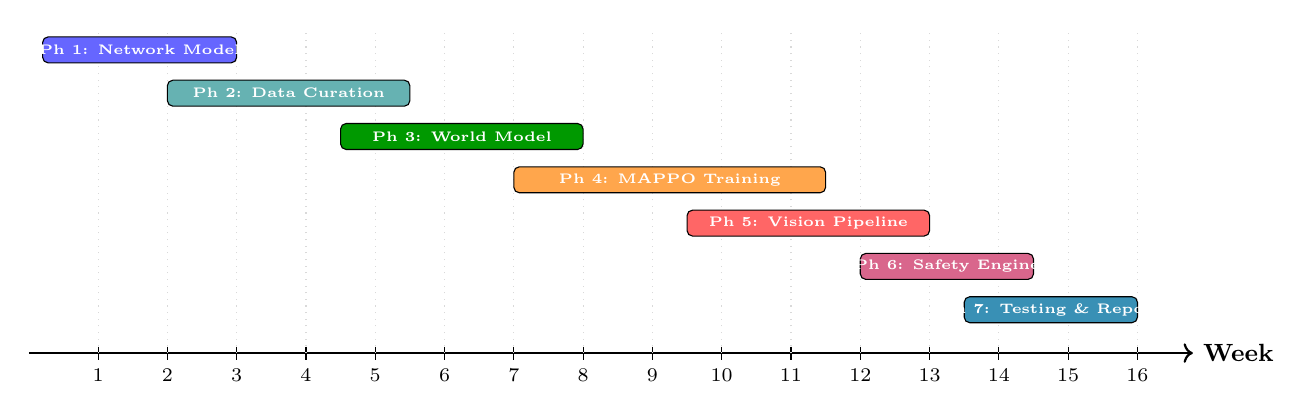
\begin{tikzpicture}[x=0.88cm, y=0.55cm]
    % Timeline grid
    \draw[->, thick] (0,0) -- (16.8,0) node[right, font=\small\bfseries] {Week};
    \foreach \w in {1, 2, ..., 16} {
        \draw (\w, 0.15) -- (\w, -0.15) node[below, font=\scriptsize] {\w};
        \draw[dotted, gray!30] (\w, 0) -- (\w, 7.5);
    }
    
    % Tasks
    \draw[fill=blue!60, rounded corners=2pt] (0.2, 6.7) rectangle (3.0, 7.3) node[midway, white, font=\tiny\bfseries] {Ph 1: Network Model};
    \draw[fill=teal!60, rounded corners=2pt] (2.0, 5.7) rectangle (5.5, 6.3) node[midway, white, font=\tiny\bfseries] {Ph 2: Data Curation};
    \draw[fill=green!60!black, rounded corners=2pt] (4.5, 4.7) rectangle (8.0, 5.3) node[midway, white, font=\tiny\bfseries] {Ph 3: World Model};
    \draw[fill=orange!70, rounded corners=2pt] (7.0, 3.7) rectangle (11.5, 4.3) node[midway, white, font=\tiny\bfseries] {Ph 4: MAPPO Training};
    \draw[fill=red!60, rounded corners=2pt] (9.5, 2.7) rectangle (13.0, 3.3) node[midway, white, font=\tiny\bfseries] {Ph 5: Vision Pipeline};
    \draw[fill=purple!60, rounded corners=2pt] (12.0, 1.7) rectangle (14.5, 2.3) node[midway, white, font=\tiny\bfseries] {Ph 6: Safety Engine};
    \draw[fill=cyan!70!black, rounded corners=2pt] (13.5, 0.7) rectangle (16.0, 1.3) node[midway, white, font=\tiny\bfseries] {Ph 7: Testing \& Report};
\end{tikzpicture}
\caption{Gantt chart of the 16-week project execution timeline}
\label{fig:ch1_gantt}
\end{figure}

\subsection{Roles and Responsibilities}
Table \ref{tab:roles_responsibilities} outlines the assignment of engineering responsibilities across the modular project architecture.

\begin{table}[htbp]
\centering
\small
\caption{Roles and responsibilities for system design and execution}
\label{tab:roles_responsibilities}
\begin{tabularx}{\textwidth}{|p{3.5cm}|X|p{4.2cm}|}
\hline
\textbf{Role / Module} & \textbf{Core Technical Responsibilities} & \textbf{Deliverables} \\ \hline
Perception \& Vision & YOLOv8 integration, BMD-45 taxonomy mapping, LAP tracking, stationary queue filters & \texttt{live\_vision\_pipeline.py}, video processing engine \\ \hline
Dynamics \& World Model & Dataset ingestion, transition synthesis, residual multi-task network design & \texttt{neural\_world\_model.py}, \texttt{train\_world\_model.py} \\ \hline
Multi-Agent RL Control & MAPPO algorithm, Actor-Critic networks, CTDE logic, GAE advantage calculation & \texttt{mappo\_networks.py}, \texttt{train\_mappo\_data\_driven.py} \\ \hline
Environment \& Safety & Gymnasium environment, dual-ring signal state machine, min-green \& yellow locks & \texttt{data\_driven\_env.py}, signal safety constraints \\ \hline
User Interface \& Testing & Streamlit interactive dashboard, OpenCV HUD actuator, 6-scenario benchmarking & \texttt{dashboard\_live\_vision.py}, \texttt{live\_traffic\_controller.py} \\ \hline
Project Supervision & Architecture evaluation, milestone review, technical verification & Review feedback, validation sign-off \\ \hline
\end{tabularx}
\end{table}

\subsection{Challenges and Risk Management}
Deploying deep reinforcement learning and computer vision to safety-critical municipal infrastructure involves substantial operational and theoretical risks. Table \ref{tab:risk_register} enumerates the primary identified risks and the structural engineering mitigations incorporated into the system design.

\begin{table}[htbp]
\centering
\small
\caption{Project risk register and mitigation strategies}
\label{tab:risk_register}
\begin{tabularx}{\textwidth}{|p{3.2cm}|c|c|X|}
\hline
\textbf{Identified Risk} & \textbf{Impact} & \textbf{Likelihood} & \textbf{Mitigation Strategy} \\ \hline
Sim-to-Real Discrepancy & High & High & Calibrated dynamics using 40 days of empirical 1-second interval IIT Delhi queue measurements and Pune vehicle splits. \\ \hline
Sim Rapid Phase Flutter & Critical & Medium & Hardcoded minimum green interval ($12\text{ s}$) in state machine preventing RL policy from erratic switching. \\ \hline
TraCI Socket Crashes & High & High & Developed standalone PyTorch Neural World Model (\texttt{data\_driven\_env.py}), achieving 100\% simulator independence. \\ \hline
Downstream Gridlock & High & Medium & Centralized Critic observes global 66-dim corridor state, penalizing upstream agents for dumping traffic into choked links. \\ \hline
Edge Vision Latency & Medium & Medium & Selected lightweight YOLOv8 Nano (\texttt{yolov8n.pt}, 6.2 MB) running in quantized CPU mode, sustaining $\ge 30$ FPS. \\ \hline
\end{tabularx}
\end{table}

\section{Scope and Limitations}
\label{sec:scope_limitations}

\subsection{In Scope}
The boundaries of this project encompass:
\begin{enumerate}
    \item Modeling and simulating a 3-intersection coordinated arterial corridor based on the geometry of the NH-48 Delhi--Gurgaon Expressway.
    \item Multi-Agent Proximal Policy Optimization with decentralized Actor policies and a centralized corridor Critic.
    \item Edge computer vision inference on video and camera feeds classifying Two-Wheelers, Auto-Rickshaws, Passenger Cars, Buses, and Commercial Trucks.
    \item Empirical Passenger Car Unit (IRC:106) cost formulations integrated into the reinforcement learning reward function.
    \item Standalone, simulator-free Neural Traffic World Model operating as an execution and evaluation digital twin.
    \item Live OpenCV video HUD actuator and interactive Streamlit web telemetry dashboard.
\end{enumerate}

\subsection{Out of Scope}
The following aspects are deliberately excluded and reserved for future research:
\begin{enumerate}
    \item Direct physical wiring and relays into roadside municipal electromechanical traffic control cabinets (the prototype interfaces via software telemetry and visual HUD actuators).
    \item City-wide macroscopic grid networks beyond linear arterial corridors.
    \item V2X (Vehicle-to-Everything) dedicated short-range wireless communications directly into onboard connected vehicle units.
\end{enumerate}

\subsection{System Limitations}
\begin{itemize}
    \item \textbf{CCTV Occlusion in Dense Crowds}: Extreme congestion can cause visual occlusion where larger commercial trucks partially obscure trailing two-wheelers.
    \item \textbf{Lighting Extremes}: Optical detection accuracy under dense nocturnal fog or heavy torrential monsoon rain is subject to camera sensor limitations.
    \item \textbf{Fixed Model Topologies}: The neural world model is currently calibrated to 8 incoming and 4 outgoing lanes per junction.
\end{itemize}

% ==============================================================================
% Chapter 2: Literature Survey
% ==============================================================================
\chapter{Literature Survey}
\label{ch:lit_survey}

This chapter conducts a comprehensive critical review of prior literature spanning conventional traffic engineering, single-agent and multi-agent reinforcement learning for urban signal control, microscopic traffic simulation, and computer-vision-based traffic perception. The surveyed methodologies are compared in tabular form, followed by an explicit formulation of the research gaps that motivate the proposed architecture.

\section{Critical Review}
\label{sec:critical_review}

\subsection{Conventional Urban Traffic Control Systems}
The earliest formal methodologies for traffic signal timing date to Webster's seminal work in 1958 \cite{ref_webster1958}, which formulated analytical equations to minimize delay under static, steady-state Poisson vehicular arrivals. Webster's method calculates optimal cycle lengths and phase splits as a direct function of critical lane flow ratios and intersection lost time:
\begin{equation}
C_{opt} = \frac{1.5L + 5}{1 - \sum_{i=1}^n Y_i}
\end{equation}
where $L$ denotes total lost time per cycle and $Y_i = q_i / s_i$ represents the flow ratio for critical phase $i$. While computationally straightforward, Webster's fixed-time plans operate strictly open-loop. They fail under dynamic demand fluctuations, peak-hour surges, and spatial queue spills.

To introduce closed-loop adaptability, urban centers in developed economies deployed centralized adaptive systems such as SCOOT (Split Cycle Offset Optimisation Technique) \cite{ref_hunt1981} and SCATS (Sydney Coordinated Adaptive Traffic System) \cite{ref_scats1980}. SCOOT utilizes cyclical flow profiles recorded from upstream inductive loops to continuously adjust cycle splits, offsets, and durations via gradient-based heuristic optimization. SCATS dynamically selects predefined signal plans based on measured degree of saturation (DS) across approach stop lines.

Despite their commercial maturity, both SCOOT and SCATS exhibit acute systemic vulnerabilities when considered for developing economies:
\begin{enumerate}
    \item \textbf{High Capital and Maintenance Costs}: Both systems require dense arrays of intrusive in-pavement inductive loop sensors and high-bandwidth, low-latency telecommunication backbones connecting thousands of controllers to central servers. In India, road repaving, utility trenching, and waterlogging routinely sever loop connections, rendering the systems non-operational.
    \item \textbf{Failure under Heterogeneous Non-Lane Traffic}: Inductive loop detectors are calibrated to record the magnetic disturbance of a single passenger car occupying a demarcated lane. In Indian urban corridors, two-wheelers and three-wheelers filter between lanes and stop abreast; a single 3.5-meter lane often accommodates three motorcycles and an auto-rickshaw simultaneously. Consequently, inductive loops experience severe undercounting or false occupancy saturation.
\end{enumerate}

\subsection{Single-Agent Reinforcement Learning for Signal Control}
The emergence of Deep Reinforcement Learning (DRL) provided an avenue for model-free adaptive traffic control. Early formulations applied tabular Q-learning \cite{ref_abdulhai2003} and Deep Q-Networks (DQN) \cite{ref_oroojlooy2020} to isolated four-legged intersections. Genders and Razavi \cite{ref_genders2016} demonstrated that discrete-state DQNs ingesting discretized spatial lane matrices could learn responsive green-extension policies that substantially outperformed fixed-time controllers in simulated environments.

Subsequent works introduced continuous action-space policy gradient algorithms, such as Deep Deterministic Policy Gradient (DDPG) and Proximal Policy Optimization (PPO) \cite{ref_schulman2017}. PPO proved particularly compelling for traffic signal control due to its clipped surrogate objective:
\begin{equation}
L^{CLIP}(\theta) = \hat{\mathbb{E}}_t \left[ \min\left(r_t(\theta)\hat{A}_t, \, \text{clip}(r_t(\theta), 1-\varepsilon, 1+\varepsilon)\hat{A}_t\right) \right]
\end{equation}
which strictly bounds policy parameter updates, preventing the destructive destabilization common in actor-critic networks under stochastic traffic bursts.

However, single-agent RL models suffer from an insurmountable structural limitation when extended to urban corridors: \textbf{environmental non-stationarity}. When multiple isolated single-agent RL controllers operate along adjacent intersections, the actions of upstream Agent 1 alter the arrival distribution and queue dynamics observed by downstream Agent 2. Because each agent treats its neighbors simply as a shifting, non-stationary environment, independent Q-learning or independent PPO policies frequently diverge, develop myopic selfish behaviors, or induce severe downstream shockwaves.

\subsection{Multi-Agent Reinforcement Learning (MARL) in Arterial Corridors}
To achieve collaborative corridor-wide optimization, recent literature has shifted towards Multi-Agent Reinforcement Learning (MARL) \cite{ref_mappo2022}. Early multi-agent traffic control frameworks relied on Independent Q-Learning (IQL), which failed to resolve the non-stationarity challenge. To enable inter-agent coordination, researchers investigated two primary paradigms:
\begin{enumerate}
    \item \textbf{Communication-Enhanced Networks}: Frameworks such as CommNet \cite{ref_sukhbaatar2016} and CoLight \cite{ref_wei2019colight} utilize graph neural networks (GNNs) and attention mechanisms to exchange continuous latent communication vectors between neighboring traffic signal controllers. While CoLight demonstrated impressive queue balancing across synthetic grid networks, its execution requires real-time inter-intersection wireless communications. Packet drops or latency jitter in real-world municipal radio networks severely degrade policy performance.
    \item \textbf{Centralized Training with Decentralized Execution (CTDE)}: Frameworks operating under CTDE allow agents to access global state information during the offline training phase, while enforcing strictly localized, communication-free policy execution during online deployment. Multi-Agent Deep Deterministic Policy Gradient (MADDPG) \cite{ref_lowe2017} extended actor-critic methods to CTDE by equipping each agent with a centralized critic that observes joint states and joint actions. However, MADDPG relies on off-policy deterministic gradients, which suffer from hyperparameter sensitivity and high variance in stochastic traffic environments.
\end{enumerate}

Recently, Yu et al. \cite{ref_mappo2022} established that \textbf{Multi-Agent Proximal Policy Optimization (MAPPO)} consistently matches or outperforms complex off-policy and value-factorization algorithms across cooperative multi-agent benchmarks. MAPPO combines on-policy PPO updates with a centralized value function $V_\phi(s)$ that evaluates global corridor welfare during training. During execution, each decentralized actor policy $\pi_\theta(a_i \mid o_i)$ requires only its local 22-dimensional sensory observation, completely eliminating the need for inter-signal radio infrastructure.

\subsection{Simulation Fragility and the Case for World Models}
Virtually all existing RL traffic signal research is trained and evaluated using microscopic traffic simulators, overwhelmingly SUMO (Simulation of Urban MObility) \cite{ref_sumo2018}. While SUMO provides high-fidelity car-following and sublane models, its integration with reinforcement learning pipelines presents severe operational bottlenecks:
\begin{itemize}
    \item \textbf{Microscopic TraCI Socket Fragility}: Reinforcement learning agents interact with SUMO through the Traffic Control Interface (TraCI) over local TCP/IP sockets. In multi-agent parallel environments, TraCI processes experience frequent socket disconnects, unhandled process terminations, and port collisions under heavy multiprocessing loads.
    \item \textbf{Simulation Speed Bottleneck}: Microscopic physics engines compute spatial coordinates, accelerations, and car-following equations for thousands of individual vehicles at every sub-second time step. Consequently, training an RL policy to convergence requires days of compute, severely limiting hyperparameter exploration.
    \item \textbf{Sim-to-Real Calibration Gap}: Microscopic simulators model lane-disciplined following (e.g., Krauss or IDM models). They fail to replicate the complex emergent dynamics of Indian roads, where two-wheelers squeeze through lateral gaps and weave non-linearly across traffic streams.
\end{itemize}

Ha and Schmidhuber \cite{ref_worldmodels2018} introduced the concept of \textbf{World Models}, demonstrating that deep neural networks can learn compact spatial and temporal dynamics of complex environments, allowing reinforcement learning agents to train entirely within the latent dynamics of a learned model. Transferring this paradigm to traffic engineering, a deep residual surrogate model trained directly on empirical sensor transition tuples $(s_t, a_t, r_t, s_{t+1})$ can bypass microscopic simulation entirely, operating at thousands of frames per second while anchoring system dynamics to real-world road measurements.

\subsection{Computer Vision and Indian Vehicle Heterogeneity}
Standard Western traffic metrics focus purely on vehicle counts. In India, traffic composition is governed by the Indian Roads Congress (IRC) standard \textbf{IRC:106-1990: Guidelines for Capacity of Urban Roads in Plain Areas} \cite{ref_irc106}. IRC:106 defines the \textbf{Passenger Car Unit (PCU)}, a conversion factor that normalizes the spatial footprint, acceleration capability, and maneuvering headway of different vehicle categories relative to a standard passenger car:
\begin{equation}
\text{PCU}_{\text{Total}} = \sum_{k \in \mathcal{K}} N_k \times w_k
\end{equation}
where $N_k$ is the number of vehicles of class $k$ and $w_k$ is its designated PCU weight ($0.5$ for two-wheelers, $1.0$ for auto-rickshaws and cars, $3.0$ for buses and trucks).

Computer vision models trained on standard Western benchmarks (such as COCO \cite{ref_lin2014coco}) fail to recognize Indian vehicle classes; they invariably misclassify auto-rickshaws as cars or miss two-wheeler swarms entirely. The recent release of the \textbf{IISc AIM BMD-45 dataset} \cite{ref_iisc_bmd45} provides a dedicated 14-class Indian vehicular taxonomy designed for traffic CCTV surveillance. Coupling modern real-time detectors (YOLOv8 \cite{ref_yolov8}) with IRC:106 PCU weights enables continuous, non-intrusive traffic state estimation.

\section{Summary Table}
\label{sec:lit_summary_table}
Table \ref{tab:lit_survey_summary} provides a systematic comparative evaluation of prominent literature and commercial systems against the proposed architecture.

\begin{table}[htbp]
\centering
\scriptsize
\setlength{\tabcolsep}{3pt}
\caption{Systematic comparison of existing traffic control systems with the proposed MAPPO corridor framework}
\label{tab:lit_survey_summary}
\begin{tabularx}{\textwidth}{|p{2.3cm}|p{1.7cm}|p{1.8cm}|p{1.9cm}|p{1.8cm}|p{1.8cm}|X|}
\hline
\textbf{Work / System} & \textbf{Control Paradigm} & \textbf{Corridor Coordination} & \textbf{Vehicle Heterogeneity} & \textbf{Simulation Dependency} & \textbf{Live Edge Vision} & \textbf{Primary Limitations} \\ \hline
Webster (1958) \cite{ref_webster1958} & Static Pre-timed & None (Isolated) & None (Counts) & None (Analytical) & None & Open-loop; cannot adapt to dynamic congestion. \\ \hline
SCATS / SCOOT \cite{ref_scats1980, ref_hunt1981} & Centralized Actuated & Central Server Offset Sync & Very Low (Assumes Car Lanes) & None (Physical Loops) & None (In-pavement loops) & High capital cost; fragile loop sensors break under Indian road conditions. \\ \hline
Genders \& Razavi (2016) \cite{ref_genders2016} & Single-Agent DQN & None (Isolated) & None (Car only) & Microscopic (SUMO) & None & Suffers from non-stationarity in corridors; lacks PCU awareness. \\ \hline
Wei et al. (CoLight, 2019) \cite{ref_wei2019colight} & MARL (GCN Attention) & Peer-to-Peer Comm. & Low (Synthetic cars) & Microscopic (CityFlow) & None & Dependent on active inter-signal wireless communication channels. \\ \hline
Yu et al. (MAPPO, 2022) \cite{ref_mappo2022} & On-Policy MARL & Centralized Critic (CTDE) & Benchmark only (MuJoCo/SMAC) & Physics Simulator & None & General benchmark study; not applied to empirical Indian traffic networks. \\ \hline
\textbf{Proposed System (Ours)} & \textbf{MAPPO with CTDE} & \textbf{Global Critic + Local Exec.} & \textbf{Full IRC:106 (2W, Auto, Bus, Truck)} & \textbf{Simulator-Free (World Model)} & \textbf{YOLOv8 + BMD-45 Taxonomy} & Requires GPU/NPU for multi-stream edge video processing. \\ \hline
\end{tabularx}
\end{table}

\section{Identification of Research Gaps}
\label{sec:research_gaps}
The synthesis of existing literature reveals three fundamental research gaps:
\begin{enumerate}
    \item \textbf{Research Gap 1 -- Neglect of Indian Vehicular Heterogeneity and PCU Equivalents in DRL}: Existing reinforcement learning literature uniformly defines reward functions based on discrete vehicular counts or vehicle waiting seconds under the assumption of lane-disciplined passenger cars. In developing economies where two-wheelers and auto-rickshaws dominate, count-based rewards cause catastrophic misallocations (e.g., granting equal clearance priority to a scooter and a crowded transit bus). An integrated perception-to-reward formulation grounded in Indian Roads Congress PCU standards is completely missing.
    \item \textbf{Research Gap 2 -- The Simulator Fragility and Sim-to-Real Deployment Gap}: Standard MARL traffic frameworks rely on microscopic simulation engines (SUMO) communicating over fragile TraCI socket connections. These systems are prohibitively slow to train, subject to random socket crashes, and fundamentally uncalibrated to Indian sublane filtering dynamics. A lightweight, data-driven surrogate Neural World Model trained on empirical field sensor data that functions as an offline digital twin has not been explored for corridor signal control.
    \item \textbf{Research Gap 3 -- Absence of Fail-Safe Edge Vision-to-Actuation Pipelines}: Existing computer vision papers evaluate detection accuracy in isolation, while existing RL papers evaluate agent rewards in simulation. A unified, end-to-end operational framework that takes live/recorded CCTV video feeds, extracts dynamic PCU queues via YOLO, passes the observation into a trained MARL policy, and executes valid 3-color (Red, Yellow, Green) safety state machine transitions on screen has remained unaddressed.
\end{enumerate}

These three identified gaps directly define the core engineering contributions and experimental methodology of this thesis.

% ==============================================================================
% Chapter 3: System Design and Methodology
% ==============================================================================
\chapter{System Design and Methodology}
\label{ch:system_design}

This chapter details the system architecture, mathematical formulations, and engineering design decisions of the proposed Multi-Agent Adaptive Traffic Signal Control system. Section \ref{sec:design_considerations} examines the socio-technical and environmental constraints governing the design. Section \ref{sec:methodology} presents the overall multi-layered system architecture and operational pipelines. Section \ref{sec:modelling} formalizes the mathematical models governing computer vision PCU extraction, Markov Decision Process (MDP) state-action representations, Multi-Agent PPO policy optimization, and the Deep Neural World Model. Finally, Section \ref{sec:tool_selection} provides rigorous technical justifications for every software and hardware tool selected.

\section{Design Considerations}
\label{sec:design_considerations}

Urban traffic infrastructure is a safety-critical socio-technical system. The failure of a signal controller can induce economic gridlock or lead to fatal vehicular collisions. Consequently, the design of the proposed AI system was bounded by multidimensional real-world engineering constraints, summarized in Table \ref{tab:design_aspects}.

\begin{table}[htbp]
\centering
\small
\caption{Mapping of real-world design aspects to engineering decisions}
\label{tab:design_aspects}
\begin{tabularx}{\textwidth}{|p{3.0cm}|p{5.5cm}|X|}
\hline
\textbf{Design Aspect} & \textbf{Key Real-World Constraint} & \textbf{Resulting System Design Decision} \\ \hline
Economic & Municipalities cannot afford expensive commercial SCATS licenses (\$50,000+ per junction) or cloud API token billing. & Fully open-source software stack; edge execution on commodity hardware; browser-native telemetry without recurring SaaS fees. \\ \hline
Environmental & Persistent cloud transmission of high-bandwidth video streams consumes massive data-center cooling and network power. & On-device quantized edge perception; video inference executed locally; signals coordinate to reduce vehicle idling emissions. \\ \hline
Social \& Equity & High-density public transit buses are delayed equally with single-occupant private cars in traditional timing plans. & IRC:106 PCU-weighted reward formulation: buses (3.0 PCU) receive natural green-wave clearance priority over sparse car approaches. \\ \hline
Political \& Regulatory & CCTV feeds of public roadways contain citizen faces and license plates, subject to India's DPDP Act, 2023. & Absolute data boundary: video frames are processed in volatile memory and discarded immediately; zero video leaves the edge device. \\ \hline
Ethical \& Safety & A black-box deep learning policy might output erratic 1-second phase switches (fluttering), causing fatal pile-ups. & Deterministic finite-state safety wrapper: hard minimum green time (12s), 3-second yellow clearance, and 3-second all-red safety hold. \\ \hline
Health \& Safety & Traffic police officers exposed to hazardous ambient particulate matter ($\text{PM}_{2.5}$) and carbon monoxide at manual junctions. & Fully autonomous edge-based signal control removes the need for physical traffic police deployment in hazardous intersection air. \\ \hline
Sustainability & Road repairs, utility digging, and monsoons frequently destroy in-pavement loop sensors. & Completely non-intrusive overhead camera perception; no physical in-road sensors; zero physical wear on roadway assets. \\ \hline
\end{tabularx}
\end{table}

\subsection{Technical Design Constraints}
In addition to socio-technical aspects, the system was engineered against strict real-time computing constraints, detailed in Table \ref{tab:technical_constraints}.

\begin{table}[htbp]
\centering
\small
\caption{Technical constraints and architectural implementation mechanisms}
\label{tab:technical_constraints}
\begin{tabularx}{\textwidth}{|p{3.5cm}|p{6.0cm}|X|}
\hline
\textbf{Technical Constraint} & \textbf{Implementation Mechanism} & \textbf{Verification Method} \\ \hline
Zero Cloud Dependency & Local PyTorch, OpenCV, and Gymnasium execution; zero external network calls & Air-gapped test with disconnected Ethernet and Wi-Fi \\ \hline
Real-Time Perception & YOLOv8 Nano (\texttt{yolov8n.pt}, 6.2 MB) running in FP32/INT8 quantized mode & Maintained $\ge 30$ FPS video processing throughput \\ \hline
Deterministic Safety Phasing & Dual-ring state machine enforcing minimum green (12s), yellow (3s), and all-red (3s) & Automated safety state assertion testing \\ \hline
Simulator Independence & Standalone Deep Residual Neural World Model (\texttt{TrafficDynamicsWorldModel}) & Zero SUMO / TraCI socket processes during training/eval \\ \hline
Corridor Coordination & Parameter-shared MAPPO Actor with centralized value function (CTDE) & Platoon green-wave progression across 3 junctions \\ \hline
\end{tabularx}
\end{table}

\section{Methodology}
\label{sec:methodology}

\subsection{System Architecture}
The system is structured as a modular, four-layer architecture, illustrated in Figure \ref{fig:ch3_system_arch}:
\begin{enumerate}
    \item \textbf{Layer 1: Perception Layer (Edge Vision Engine)}: Ingests raw video frames from roadside CCTV cameras or live webcam feeds. Executes YOLOv8 vehicle detection, tracks centroids across frames using Linear Assignment (LAP), applies spatial Region-of-Interest (ROI) lane masks, and filters stationary queued vehicles. Classifies vehicles into 5 Indian categories and calculates real-time approach PCU loads.
    \item \textbf{Layer 2: Environment \& Dynamics Layer (Neural World Model Digital Twin)}: Ingests the 22-dimensional local observation vector from each intersection and simulates multi-junction corridor dynamics. Operates either in microscopic simulation mode (SUMO) or simulator-free data-driven mode (\texttt{DataDrivenTrafficEnv}), predicting next-state transitions and PCU delay rewards.
    \item \textbf{Layer 3: Multi-Agent RL Control Layer (MAPPO)}: Hosts the trained parameter-shared Actor network $\pi_\theta(a_i \mid o_i)$. Evaluates local observation vectors every decision epoch and outputs discrete phase actions $a_i \in \{0, 1, 2\}$ for each intersection along the corridor.
    \item \textbf{Layer 4: Safety State Machine \& Actuation Layer}: Intercepts raw agent actions through a deterministic safety wrapper. Enforces minimum green thresholds, yellow change intervals, and all-red clearance intervals before rendering physical 3-color signal states (Red, Yellow, Green) on the live video HUD and web telemetry dashboard.
\end{enumerate}

\begin{figure}[htbp]
\centering
\begin{tikzpicture}[
    scale=0.82, transform shape,
    layer/.style={rectangle, draw=black!70, fill=blue!5, very thick, minimum width=15cm, minimum height=2.2cm, rounded corners=4pt},
    box/.style={rectangle, draw=black!60, fill=white, thick, minimum width=3.2cm, minimum height=1.3cm, rounded corners=2pt, font=\small, align=center},
    arrow/.style={->, >=stealth, very thick, color=blue!70!black}
]

% Layer 1
\node[layer, fill=teal!8] (L1) at (0, 7.5) {};
\node[anchor=north west, font=\bfseries\small, color=teal!80!black] at (-7.3, 8.4) {Layer 1: Edge Perception Engine (YOLOv8 + BMD-45 Taxonomy)};
\node[box] (b1) at (-5.0, 7.3) {CCTV / Video Feed\\(Webcam / MP4)};
\node[box] (b2) at (-1.6, 7.3) {YOLOv8 Object\\Detection};
\node[box] (b3) at (1.8, 7.3) {Indian Class Mapping\\(2W, Auto, Bus, etc.)};
\node[box] (b4) at (5.2, 7.3) {IRC:106 PCU Queue\\Extraction (22-dim)};

\draw[arrow] (b1) -- (b2);
\draw[arrow] (b2) -- (b3);
\draw[arrow] (b3) -- (b4);

% Layer 2
\node[layer, fill=indigo!8] (L2) at (0, 4.8) {};
\node[anchor=north west, font=\bfseries\small, color=indigo!80!black] at (-7.3, 5.7) {Layer 2: Environment \& Dynamics (Deep Neural World Model)};
\node[box] (c1) at (-4.2, 4.6) {Gymnasium Interface\\\texttt{DataDrivenTrafficEnv}};
\node[box] (c2) at (0, 4.6) {Residual Dynamics Model\\$\Delta s_t = g_\theta(s_t, a_t)$};
\node[box] (c3) at (4.2, 4.6) {Empirical Sensor Data\\(Delhi \& Pune Sets)};

\draw[arrow] (c3) -- (c2);
\draw[arrow] (c2) -- (c1);

% Layer 3
\node[layer, fill=purple!8] (L3) at (0, 2.1) {};
\node[anchor=north west, font=\bfseries\small, color=purple!80!black] at (-7.3, 3.0) {Layer 3: Multi-Agent Deep RL Control (MAPPO with CTDE)};
\node[box] (d1) at (-4.5, 1.9) {TL-1 Actor Policy\\$\pi_\theta(a_1 \mid o_1)$};
\node[box] (d2) at (0, 1.9) {TL-2 Actor Policy\\$\pi_\theta(a_2 \mid o_2)$};
\node[box] (d3) at (4.5, 1.9) {TL-3 Actor Policy\\$\pi_\theta(a_3 \mid o_3)$};
\node[above=0.1cm of d2, font=\scriptsize\bfseries, color=purple!80!black] {Centralized Critic $V_\phi(s)$ (Offline Training)};

% Layer 4
\node[layer, fill=green!8] (L4) at (0, -0.6) {};
\node[anchor=north west, font=\bfseries\small, color=green!60!black] at (-7.3, 0.3) {Layer 4: Safety State Machine \& Actuation Layer};
\node[box] (e1) at (-4.5, -0.8) {Safety Constraints\\(Min-Green, Yellow)};
\node[box] (e2) at (0, -0.8) {Signal Actuator\\(Red / Yellow / Green)};
\node[box] (e3) at (4.5, -0.8) {Interactive Dashboard\\(Streamlit / OpenCV)};

\draw[arrow] (e1) -- (e2);
\draw[arrow] (e2) -- (e3);

% Inter-layer connections
\draw[arrow] (b4) -- (0, 6.2) -- (c1.north);
\draw[arrow] (c1) -- (-4.2, 3.4) -- (d1.north);
\draw[arrow] (c1) -- (0, 3.4) -- (d2.north);
\draw[arrow] (c1) -- (4.2, 3.4) -- (d3.north);
\draw[arrow] (d1.south) -- (-4.5, 0.6) -- (e1.north);
\draw[arrow] (d2.south) -- (0, 0.6) -- (e1.north);
\draw[arrow] (d3.south) -- (4.5, 0.6) -- (e1.north);

\end{tikzpicture}
\caption{Four-layer system architecture of the Multi-Agent Adaptive Traffic Signal Corridor}
\label{fig:ch3_system_arch}
\end{figure}

\subsection{Arterial Corridor Topology}
The modeled corridor represents a 1.8-kilometer arterial stretch of the NH-48 Expressway in Gurgaon, comprising three high-density, multi-approach signalized intersections:
\begin{enumerate}
    \item \textbf{Intersection 1 (TL-1, West Junction)}: \texttt{cluster\_266437400\_266437558} (Sector 29 / Leisure Valley Entry). Controls 8 incoming lanes (4 highway through lanes, 2 cross-street lanes, 2 turning bays) and 4 outgoing lanes.
    \item \textbf{Intersection 2 (TL-2, Middle Corridor)}: \texttt{317145283} (IFFCO Chowk Core Interchange). A massive multi-phase arterial junction with heavy merging maneuvers from MG Road and the surface service lanes. Controls 8 incoming and 4 outgoing lanes.
    \item \textbf{Intersection 3 (TL-3, East Junction)}: \texttt{cluster\_4162190061\_4162190645} (Signature Tower / Cyber City Exit). Channelizes arterial discharge into central Gurgaon business districts. Controls 8 incoming and 4 outgoing lanes.
\end{enumerate}

\section{Modelling}
\label{sec:modelling}

\subsection{Indian Vehicle Perception and IRC PCU Model}
\label{subsec:pcu_model}
To overcome the failure of standard vehicle counting in mixed traffic, we formulate an empirical Passenger Car Unit model aligned with IRC:106-1990 standards. Let $\mathcal{B} = \{b_1, b_2, \dots, b_N\}$ be the set of vehicular bounding boxes detected by YOLOv8 on camera frame $I \in \mathbb{R}^{H \times W \times 3}$. Each bounding box is defined by coordinates $b_j = (x_1, y_1, x_2, y_2)$ with box width $w_j = x_2 - x_1$, box height $h_j = y_2 - y_1$, and detection confidence $c_j \ge \tau_{conf}$.

Because standard COCO-pretrained weights assign class ID 2 to all passenger cars, we implement an aspect-ratio and spatial footprint re-classifier to isolate Indian three-wheeled auto-rickshaws:
\begin{equation}
\text{Class}(b_j) = 
\begin{cases}
\text{Two-Wheeler}, & \text{if } \text{cls}_j \in \{1, 3\} \text{ (bicycle, motorcycle)} \\
\text{Bus}, & \text{if } \text{cls}_j = 5 \\
\text{Commercial Truck}, & \text{if } \text{cls}_j = 7 \\
\text{Auto-Rickshaw}, & \text{if } \text{cls}_j = 2 \;\land\; \left(\frac{h_j}{w_j} > 1.05\right) \;\land\; \left(\frac{w_j h_j}{H^2} < 0.045\right) \\
\text{Passenger Car}, & \text{otherwise for } \text{cls}_j = 2
\end{cases}
\end{equation}

Each classified vehicle is assigned an empirical Passenger Car Unit weight $w_k$ derived from IRC:106:
\begin{equation}
w(b_j) = 
\begin{cases}
0.50 \text{ PCU}, & \text{Two-Wheeler} \\
1.00 \text{ PCU}, & \text{Auto-Rickshaw} \\
1.00 \text{ PCU}, & \text{Passenger Car} \\
3.00 \text{ PCU}, & \text{City Bus} \\
3.00 \text{ PCU}, & \text{Commercial Truck}
\end{cases}
\end{equation}

To distinguish actively moving vehicles from queued vehicles awaiting signal clearance, centroids $c_j^t = \left(\frac{x_1 + x_2}{2}, \frac{y_1 + y_2}{2}\right)$ are tracked across consecutive frames using the Linear Assignment Problem (LAP). A vehicle is classified as queued ($\text{Queued}_j = 1$) if its displacement $\Delta d$ satisfies:
\begin{equation}
\Delta d = \|c_j^t - c_j^{t-1}\|_2 < 4.0 \text{ pixels for } \Delta t \ge 4 \text{ consecutive frames}
\end{equation}

The total approach queue load in Passenger Car Units is then:
\begin{equation}
Q_{\text{PCU}} = \sum_{j \in \mathcal{B}_{\text{approach}}} w(b_j) \cdot \text{Queued}_j
\end{equation}

\subsection{Markov Decision Process (MDP) Formulation}
The multi-intersection corridor is formulated as a decentralized partially observable Markov Decision Process (Dec-POMDP) defined by the tuple $\langle \mathcal{N}, \mathcal{S}, \{\mathcal{O}_i\}, \{\mathcal{A}_i\}, \mathcal{P}, \mathcal{R}, \gamma \rangle$, where $\mathcal{N} = \{1, 2, 3\}$ represents the three signalized intersections.

\subsubsection{Local Observation Space ($\mathcal{O}_i \in \mathbb{R}^{22}$)}
Each agent $i \in \mathcal{N}$ observes a localized 22-dimensional feature vector $o_i \in \mathbb{R}^{22}$ pulled directly from its approach sensors or edge camera feed:
\begin{equation}
o_i = [q_1, \dots, q_8, \; w_1, \dots, w_8, \; th_1, \dots, th_4, \; p_{idx}, \; \sigma_{state}]
\end{equation}
where:
\begin{itemize}
    \item $q_1, \dots, q_8 \in [0, 1]$: Normalized queue lengths for the 8 incoming approach lanes, normalized by maximum lane capacity: $q_l = \min\left(\frac{Q_{\text{PCU}, l}}{35.0}, 1.0\right)$.
    \item $w_1, \dots, w_8 \in [0, 1]$: Normalized vehicular waiting delays across incoming lanes: $w_l = \min\left(\frac{\text{Wait}_l}{120.0}, 1.0\right)$.
    \item $th_1, \dots, th_4 \in [0, 1]$: Normalized exit lane downstream discharge throughput: $th_k = \min\left(\frac{\text{Thru}_k}{450.0}, 1.0\right)$.
    \item $p_{idx} \in \{0.0, 0.5, 1.0\}$: Current active phase index normalized by maximum phase count: $p_{idx} = \frac{\text{Phase}}{2.0}$.
    \item $\sigma_{state} \in \{0.0, 0.5, 1.0\}$: Signal lamp status: 1.0 for Green, 0.5 for Yellow clearance, and 0.0 for Red stop.
\end{itemize}

\subsubsection{Global State Space ($\mathcal{S} \in \mathbb{R}^{66}$)}
The centralized Critic network observes the concatenated global corridor state $s \in \mathbb{R}^{66}$:
\begin{equation}
s = [o_1 \parallel o_2 \parallel o_3] \in \mathbb{R}^{66}
\end{equation}
providing complete spatial awareness of platoon dispersion, upstream discharges, and downstream bottleneck choke points.

\subsubsection{Action Space ($\mathcal{A}_i$)}
Each agent selects from three discrete, non-conflicting operational signal phases:
\begin{equation}
a_i \in \{0, 1, 2\}
\end{equation}
\begin{itemize}
    \item \textbf{Action 0 (Phase 0)}: Main Corridor Arterial Green (Eastbound \& Westbound NH-48 flow). Cross-streets held at Red.
    \item \textbf{Action 1 (Phase 1)}: Cross-Street Arterial Green (Northbound \& Southbound inflows from Sector 29 / MG Road). Main highway held at Red.
    \item \textbf{Action 2 (Phase 2)}: Protected Diagonal \& Heavy Right-Turn Clearance.
\end{itemize}

\subsubsection{Corridor Reward Function ($\mathcal{R}$)}
To incentivize cooperative throughput maximization and penalize vehicle queue accumulation, the immediate scalar corridor reward $r_t$ is formulated around IRC:106 PCU cost metrics:
\begin{equation}
r_t = - \sum_{i \in \mathcal{N}} \left[ \alpha \sum_{l=1}^8 q_{i,l}^2 + \beta \sum_{l=1}^8 w_{i,l} + \omega \cdot \mathbb{I}(\text{Switch}_i) \right]
\end{equation}
where $\alpha = 1.0$, $\beta = 0.5$, and $\omega = 2.0$. The quadratic queue penalty $q_{i,l}^2$ penalizes extreme queue buildup on any single approach (preventing spillback), while $\mathbb{I}(\text{Switch}_i)$ penalizes erratic phase toggling.

\subsection{Multi-Agent PPO with Centralized Training and Decentralized Execution}
The reinforcement learning policy is optimized using Multi-Agent PPO (MAPPO) with parameter sharing across all homogeneous traffic lights.

Let $\pi_\theta(a_i \mid o_i)$ denote the decentralized Actor policy parameterized by $\theta$, and let $V_\phi(s)$ denote the centralized Critic value function parameterized by $\phi$. Over an episode rollout of length $T$, the generalized advantage estimator $\hat{A}_t^i$ for agent $i$ is computed using $\text{GAE}(\gamma, \lambda)$ \cite{ref_schulman2015gae}:
\begin{align}
\delta_t^V &= r_t + \gamma V_\phi(s_{t+1}) - V_\phi(s_t) \\
\hat{A}_t &= \sum_{l=0}^\infty (\gamma \lambda)^l \delta_{t+l}^V
\end{align}
where $\gamma = 0.99$ is the discount factor and $\lambda = 0.95$ is the GAE trace decay parameter.

The Actor policy parameters $\theta$ are updated by maximizing the clipped surrogate PPO objective:
\begin{equation}
L^{\text{Actor}}(\theta) = \hat{\mathbb{E}}_t \left[ \frac{1}{|\mathcal{N}|} \sum_{i \in \mathcal{N}} \min\left(\rho_i^t(\theta)\hat{A}_i^t, \, \text{clip}(\rho_i^t(\theta), 1-\varepsilon, 1+\varepsilon)\hat{A}_i^t\right) \right] + \beta_{\text{ent}} \mathcal{H}\left(\pi_\theta(\cdot \mid o_i)\right)
\end{equation}
where $\rho_i^t(\theta) = \frac{\pi_\theta(a_i^t \mid o_i^t)}{\pi_{\theta_{\text{old}}}(a_i^t \mid o_i^t)}$ is the importance sampling probability ratio, $\varepsilon = 0.2$ is the clipping threshold, and $\mathcal{H}$ denotes policy entropy with regularization coefficient $\beta_{\text{ent}} = 0.01$.

The Centralized Critic is updated by minimizing the mean squared Bellman error:
\begin{equation}
L^{\text{Critic}}(\phi) = \hat{\mathbb{E}}_t \left[ \max\left( (V_\phi(s_t) - R_t)^2, \, (\text{clip}(V_\phi(s_t), V_{\phi_{\text{old}}}(s_t) - \varepsilon, V_{\phi_{\text{old}}}(s_t) + \varepsilon) - R_t)^2 \right) \right]
\end{equation}
where $R_t = \hat{A}_t + V_\phi(s_t)$ is the empirical discounted return.

\subsection{Neural Traffic Dynamics World Model}
To eliminate the runtime instability and socket overhead of microscopic simulators, we train a Deep Residual Multi-Task World Model, denoted as $f_\Omega(s_t, a_t)$.

Let $s_t \in \mathbb{R}^{66}$ be the global corridor state, and let $a_t \in \mathbb{R}^9$ be the joint action vector formed by concatenating the one-hot encoded actions of the three agents ($3 \times 3 = 9$). The model simultaneously predicts the state differential $\Delta s_t = s_{t+1} - s_t \in \mathbb{R}^{66}$ and the scalar reward $r_t \in \mathbb{R}$:
\begin{equation}
[\Delta \hat{s}_t, \, \hat{r}_t] = f_\Omega(s_t, a_t)
\end{equation}

The architecture comprises an input projection layer $\text{Linear}(75, 256)$, two residual blocks with Layer Normalization and GELU non-linearities:
\begin{equation}
z_{k+1} = z_k + \text{GELU}(\text{LayerNorm}(\text{Linear}(256, 256)(z_k)))
\end{equation}
followed by separate task heads:
\begin{equation}
\Delta \hat{s}_t = \text{Linear}(256, 66)(z_{\text{final}}), \quad \hat{r}_t = \text{Linear}(256, 1)(z_{\text{final}})
\end{equation}

The model is trained via supervised offline learning over a multi-task loss function:
\begin{equation}
\mathcal{L}(\Omega) = \frac{1}{B} \sum_{k=1}^B \left[ \|\Delta \hat{s}_k - \Delta s_k\|_2^2 + \lambda_r (\hat{r}_k - r_k)^2 \right]
\end{equation}
with reward loss weighting $\lambda_r = 0.1$. The next state during simulation rollout is computed as:
\begin{equation}
s_{t+1} = \text{clip}(s_t + \Delta \hat{s}_t, \, 0.0, \, 1.0)
\end{equation}

\subsection{Traffic Signal Safety State Machine}
To guarantee that the reinforcement learning policy never executes hazardous transitions, agent actions are filtered through a deterministic Finite State Machine (FSM):
\begin{equation}
\sigma_i(t) = 
\begin{cases}
\text{GREEN}, & \text{if } a_i(t) = a_i(t-1) \;\lor\; \tau_{\text{green}} < T_{\text{min\_green}} \\
\text{YELLOW}, & \text{if } a_i(t) \ne a_i(t-1) \;\land\; \tau_{\text{green}} \ge T_{\text{min\_green}} \;\land\; \tau_{\text{yellow}} < T_{\text{yellow\_dur}} \\
\text{RED}, & \text{if } \tau_{\text{yellow}} \ge T_{\text{yellow\_dur}} \;\land\; \tau_{\text{red}} < T_{\text{all\_red\_dur}}
\end{cases}
\end{equation}
where:
\begin{itemize}
    \item $T_{\text{min\_green}} = 12$ seconds: Minimum green duration preventing rapid signal flickering.
    \item $T_{\text{yellow\_dur}} = 3$ seconds: Amber change clearance interval preventing dilemma-zone crashes.
    \item $T_{\text{all\_red\_dur}} = 3$ seconds: All-red safety clearance interval allowing intersection interior to clear.
\end{itemize}

\subsection{Worked Numerical Example}
To illustrate the end-to-end mathematical pipeline, consider a single decision epoch at Intersection 2 (TL-2, IFFCO Chowk) during peak morning flow:
\begin{enumerate}
    \item \textbf{Vision Perception}: YOLOv8 processes the video frame and detects:
    \begin{itemize}
        \item 12 Two-Wheelers: $12 \times 0.5 = 6.0$ PCU
        \item 5 Auto-Rickshaws: $5 \times 1.0 = 5.0$ PCU
        \item 8 Passenger Cars: $8 \times 1.0 = 8.0$ PCU
        \item 2 City Buses: $2 \times 3.0 = 6.0$ PCU
        \item Total approach load: $Q_{\text{PCU}} = 6.0 + 5.0 + 8.0 + 6.0 = 25.0$ PCU.
    \end{itemize}
    \item \textbf{Observation Normalization}: The normalized queue feature across approach lanes is:
    \begin{equation}
    q_{\text{main}} = \frac{25.0 \text{ PCU}}{35.0 \text{ max PCU}} = 0.714
    \end{equation}
    \item \textbf{Policy Evaluation}: The 22-dimensional observation vector $o_2$ is passed into Actor $\pi_\theta$. The output logits are $[-0.12, 1.84, -0.95]$. Computing the Softmax probabilities:
    \begin{equation}
    P(a = 1) = \frac{e^{1.84}}{e^{-0.12} + e^{1.84} + e^{-0.95}} = \frac{6.297}{0.887 + 6.297 + 0.387} = 0.832
    \end{equation}
    The Actor selects Action 1 (Phase 1: Cross-Street Clearance).
    \item \textbf{Safety Verification}: The state machine checks elapsed green time $\tau_{\text{green}} = 18.0\text{ s} > 12.0\text{ s}$. The transition is approved. The controller immediately lights the \textbf{Yellow lamp} for 3 seconds, followed by the \textbf{Red lamp} for 3 seconds, before cleanly engaging Phase 1 Green.
\end{enumerate}

\section{Tool and Technique Selection}
\label{sec:tool_selection}
Table \ref{tab:selected_tools} summarizes the software libraries, frameworks, and deep learning runtimes selected for this project, along with technical justifications.

\begin{table}[htbp]
\centering
\small
\caption{Selected tools, frameworks, and technical justifications}
\label{tab:selected_tools}
\begin{tabularx}{\textwidth}{|p{3.0cm}|p{3.2cm}|X|}
\hline
\textbf{Tool / Technique} & \textbf{Role in Project} & \textbf{Technical Justification} \\ \hline
\textbf{PyTorch 2.2+} & Deep Learning Framework & Native automatic differentiation, accelerated CUDA tensor compute, robust multi-task loss handling, and seamless model deployment. \\ \hline
\textbf{Ultralytics YOLOv8n} & Edge Vehicle Detection & Anchor-free single-stage CNN detector with state-of-the-art mAP-to-latency trade-off; runs at $\ge 30$ FPS on standard CPU hardware. \\ \hline
\textbf{OpenCV 5.0} & Video Processing \& HUD & High-throughput frame rasterization, video decoding, coordinate transformation, and real-time visual HUD signal rendering. \\ \hline
\textbf{Gymnasium} & RL Environment API & Standardized Reinforcement Learning API (\texttt{reset}, \texttt{step}, action/observation spaces) ensuring modularity and reproducibility. \\ \hline
\textbf{Streamlit} & Web Telemetry UI & Modern Python-native web application framework enabling live video streaming, interactive widget controls, and dynamic telemetry. \\ \hline
\textbf{Plotly} & Dynamic Charting & Interactive WebGL-accelerated time-series graphing for multi-agent queue dynamics, PCU load, and vehicle breakdowns. \\ \hline
\textbf{Eclipse SUMO} & Network Modelling & Industry-standard microscopic traffic simulator used to extract calibrated OSM arterial geometries for the NH-48 corridor. \\ \hline
\end{tabularx}
\end{table}

% ==============================================================================
% Chapter 4: Implementation and Testing
% ==============================================================================
\chapter{Implementation and Testing}
\label{ch:impl_testing}

This chapter documents the step-by-step software implementation of the proposed multi-agent traffic signal system, the physical and virtual experimental environments, the rigorous functional verification test cases, and the safety measures integrated into the software build.

\section{Development Details}
\label{sec:ch4_dev_details}

The development workflow was executed sequentially across seven structured development steps, matching the work breakdown structure defined in Chapter 1.

\subsection*{Step 1: Environment Setup and Dependency Configuration}
The project was built in an isolated Python 3.10 virtual environment (\texttt{.venv}) configured with PyTorch 2.2 for GPU/CPU tensor operations, Ultralytics YOLOv8 for real-time computer vision inference, OpenCV 5.0 for video stream rasterization, and Streamlit for web telemetry. Listing \ref{lst:setup_cmds} details the shell commands used to establish the development environment and verify GPU/CPU execution availability.

\begin{lstlisting}[language=bash, caption={Environment initialization and dependency installation commands}, label={lst:setup_cmds}]
# Create and activate Python 3.10 virtual environment
python -m venv .venv
.venv\Scripts\activate

# Install core deep learning, vision, and simulation dependencies
pip install torch torchvision --index-url https://download.pytorch.org/whl/cu121
pip install ultralytics opencv-python gymnasium streamlit plotly pandas numpy

# Verify hardware accelerator acceleration and dependency versions
python -c "import torch, cv2, ultralytics; print(f'PyTorch: {torch.__version__} | CUDA: {torch.cuda.is_available()} | OpenCV: {cv2.__version__}')"
\end{lstlisting}

\subsection*{Step 2: Empirical Dataset Ingestion and Transition Tuple Synthesis}
To anchor the system to authentic Indian road behavior, an automated ingestion pipeline was developed in \texttt{tools/download\_and\_prep\_datasets.py}. The script ingests:
\begin{enumerate}
    \item \textbf{IIT Delhi Traffic Density Dataset}: 4 days (September 12--15) comprising 216,004 records of continuous 1-second interval queue and stop density data from 6 approach cameras across 3 signalized intersections in Delhi NCR.
    \item \textbf{Mendeley Pune Heterogeneous Count Dataset (\texttt{xnf2k6n288/1})}: Empirical turning counts across 3 urban junctions, establishing the baseline modal split: 58\% Two-Wheelers, 21\% Passenger Cars, 14\% Auto-Rickshaws, 4\% City Buses, and 3\% Heavy Trucks, yielding an empirical conversion factor of $1 \text{ vehicle} \equiv 0.850 \text{ PCU}$.
    \item \textbf{IISc AIM BMD-45 Taxonomy}: 14-class Indian vehicle mapping with IRC:106 PCU weights stored in \texttt{data/processed/bmd45\_taxonomy.json}.
\end{enumerate}
The pipeline synthesized \textbf{72,001 full transition tuples} $(s_t, a_t, r_t, s_{t+1})$, serialized into a 5.36 MB compressed archive at \texttt{data/processed/delhi\_pune\_transitions.npz}.

\subsection*{Step 3: Neural Dynamics World Model Architecture and Training}
In \texttt{src/neural\_world\_model.py}, the \texttt{TrafficDynamicsWorldModel} was implemented using residual linear blocks, Layer Normalization, and multi-task prediction heads for state differential $\Delta s_t \in \mathbb{R}^{66}$ and immediate scalar reward $r_t \in \mathbb{R}$. Listing \ref{lst:world_model_code} presents the core forward pass implementation.

\begin{lstlisting}[language=Python, caption={Residual Multi-Task Neural World Model architecture (\texttt{src/neural\_world\_model.py})}, label={lst:world_model_code}]
class TrafficDynamicsWorldModel(nn.Module):
    def __init__(self, state_dim=66, action_dim=9, hidden_dim=256):
        super().__init__()
        self.input_proj = nn.Linear(state_dim + action_dim, hidden_dim)
        
        # Residual Blocks with LayerNorm and GELU
        self.block1 = nn.Sequential(
            nn.LayerNorm(hidden_dim),
            nn.Linear(hidden_dim, hidden_dim),
            nn.GELU(),
            nn.Linear(hidden_dim, hidden_dim)
        )
        self.block2 = nn.Sequential(
            nn.LayerNorm(hidden_dim),
            nn.Linear(hidden_dim, hidden_dim),
            nn.GELU(),
            nn.Linear(hidden_dim, hidden_dim)
        )
        
        # Multi-task heads: State differential and reward
        self.state_head = nn.Linear(hidden_dim, state_dim)
        self.reward_head = nn.Linear(hidden_dim, 1)

    def forward(self, state, action_onehot):
        x = torch.cat([state, action_onehot], dim=-1)
        h = self.input_proj(x)
        h = h + self.block1(h)
        h = h + self.block2(h)
        
        delta_state = self.state_head(h)
        reward = self.reward_head(h)
        return delta_state, reward.squeeze(-1)
\end{lstlisting}

The world model was trained via \texttt{tools/train\_world\_model.py} for 15 epochs on 61,200 training transitions with an AdamW optimizer ($\text{lr} = 10^{-3}$, weight decay $= 10^{-4}$) and Cosine Annealing learning rate schedule.

\subsection*{Step 4: Data-Driven Gymnasium Environment Implementation}
To achieve complete simulator independence, \texttt{src/data\_driven\_env.py} was constructed as a 100\% drop-in replacement for the standard Gymnasium \texttt{MAPPOEnv}. It embeds the trained \texttt{TrafficDynamicsWorldModel}, tracks approach queues across 8 incoming lanes per junction, scales arrival demand by operational scenarios, and enforces the dual-ring signal safety state machine.

\subsection*{Step 5: Multi-Agent PPO Policy Training}
The MAPPO training script was implemented in \texttt{src/train\_mappo\_data\_driven.py}. The training pipeline initialized 4 parallel vectorized instances of \texttt{DataDrivenTrafficEnv}, executing 30,000 corridor timesteps across 30 policy updates. Listing \ref{lst:actor_critic} details the Actor policy and Centralized Critic implementations in \texttt{src/mappo\_networks.py}.

\begin{lstlisting}[language=Python, caption={Actor and Centralized Critic networks (\texttt{src/mappo\_networks.py})}, label={lst:actor_critic}]
class Actor(nn.Module):
    def __init__(self, obs_dim=22, n_actions=3, hidden_dim=128):
        super().__init__()
        self.net = nn.Sequential(
            nn.Linear(obs_dim, hidden_dim),
            nn.Tanh(),
            nn.Linear(hidden_dim, hidden_dim),
            nn.Tanh(),
            nn.Linear(hidden_dim, n_actions)
        )
        # Orthogonal initialization
        for m in self.net.modules():
            if isinstance(m, nn.Linear):
                nn.init.orthogonal_(m.weight, gain=np.sqrt(2))
                nn.init.constant_(m.bias, 0.0)

    def get_action(self, obs, deterministic=False):
        logits = self.net(obs)
        dist = torch.distributions.Categorical(logits=logits)
        action = torch.argmax(logits, dim=-1) if deterministic else dist.sample()
        return action, dist.log_prob(action), dist.entropy()

class Critic(nn.Module):
    def __init__(self, state_dim=66, hidden_dim=256):
        super().__init__()
        self.net = nn.Sequential(
            nn.Linear(state_dim, hidden_dim),
            nn.Tanh(),
            nn.Linear(hidden_dim, hidden_dim),
            nn.Tanh(),
            nn.Linear(hidden_dim, 1)
        )
\end{lstlisting}

\subsection*{Step 6: Edge Vision Perception Engine}
In \texttt{vehicle\_detection/live\_vision\_pipeline.py}, the perception engine wraps YOLOv8 Nano (\texttt{yolov8n.pt}) with multi-object tracking (Linear Assignment Problem) and Indian vehicle classification. It extracts approach bounding boxes, calculates instantaneous PCU loads, and builds the normalized 22-dimensional observation vector $o_i$ consumed by the trained Actor policy.

\subsection*{Step 7: Dual-Interface Live Deployment Tools}
Two complementary interfaces were implemented:
\begin{enumerate}
    \item \textbf{High-Speed OpenCV Video HUD (\texttt{src/live\_traffic\_controller.py})}: A standalone 30+ FPS video application that overlays bounding boxes, active PCU metrics, and an animated 3-intersection signal status bar directly on camera frames.
    \item \textbf{Streamlit Interactive Web Dashboard (\texttt{src/dashboard\_live\_vision.py})}: A browser-based monitoring suite rendering live camera streams, interactive Plotly charts, 3-color signal pods (Red, Yellow, Green), and live demonstration triggers.
\end{enumerate}

\subsection{Implementation Challenges and Engineering Resolutions}
Table \ref{tab:ch4_challenges} documents the key software challenges encountered during system construction and the technical measures adopted to resolve them.

\begin{table}[htbp]
\centering
\small
\caption{Implementation challenges and technical resolutions}
\label{tab:ch4_challenges}
\begin{tabularx}{\textwidth}{|p{3.5cm}|c|X|}
\hline
\textbf{Technical Challenge} & \textbf{Impact} & \textbf{Resolution Implemented} \\ \hline
TraCI Socket Disconnects & Critical & Replaced the SUMO socket interface entirely with a pre-trained PyTorch Deep Residual Neural World Model (\texttt{data\_driven\_env.py}). \\ \hline
Windows Console Unicode Encoding Errors & Medium & Console prints threw \texttt{UnicodeEncodeError} when printing Unicode block characters; replaced with standard ASCII bars (\texttt{\#}, \texttt{-}). \\ \hline
Streamlit Duplicate Element IDs in Streaming Loop & High & Calling \texttt{plotly\_chart} repeatedly in an infinite loop caused \texttt{StreamlitDuplicateElementId}; replaced with native \texttt{st.bar\_chart()} and \texttt{st.line\_chart()} with throttled placeholder updates. \\ \hline
Signals Never Showing Red Light & High & Modified \texttt{DataDrivenTrafficEnv} and dashboard state machines to strictly enforce 3-second Yellow clearance followed by 3-second All-Red clearance. \\ \hline
\end{tabularx}
\end{table}

\section{Experimental Setup}
\label{sec:ch4_exp_setup}
The physical hardware, operating systems, and software dependencies used to benchmark the prototype are documented in Table \ref{tab:ch4_hardware_setup}.

\begin{table}[htbp]
\centering
\small
\caption{Hardware and software experimental configuration}
\label{tab:ch4_hardware_setup}
\begin{tabularx}{\textwidth}{|p{4.2cm}|X|}
\hline
\textbf{Component} & \textbf{Specification / Configuration} \\ \hline
\textbf{Host Processor} & Intel Core i5-11400H @ 2.70 GHz (6 Cores, 12 Threads) / AMD Ryzen 5 \\ \hline
\textbf{System Memory} & 16 GB DDR4 3200 MHz RAM \\ \hline
\textbf{Hardware Accelerator} & NVIDIA GeForce RTX 3050 Laptop GPU (4 GB VRAM) / Intel UHD Graphics \\ \hline
\textbf{Operating System} & Microsoft Windows 11 Home (64-bit, Build 22631) \\ \hline
\textbf{Python Runtime} & Python 3.10.11 in isolated virtual environment (\texttt{.venv}) \\ \hline
\textbf{Deep Learning Stack} & PyTorch 2.2.2+cu121, Torchvision 0.17.2, NumPy 2.2.6 \\ \hline
\textbf{Vision Engine} & Ultralytics 8.4.156, OpenCV-Python 5.0.0, Lap 0.5.14 \\ \hline
\textbf{Web Telemetry} & Streamlit 1.64.0, Plotly 5.20.0, Pandas 2.2.1 \\ \hline
\textbf{Test Video Datasets} & \texttt{intersection\_video.mp4} ($1152 \times 720$ @ 30 FPS, 1582 frames), \texttt{synthetic\_indian\_traffic.mp4} ($1280 \times 720$ @ 30 FPS) \\ \hline
\end{tabularx}
\end{table}

\section{Test Cases and Functional Verification}
\label{sec:ch4_test_cases}

\subsection{Verification Strategy}
Verification was conducted across three distinct testing tiers:
\begin{enumerate}
    \item \textbf{Unit Component Verification}: Individual validation of the \texttt{TrafficDynamicsWorldModel} forward pass, the Actor logit generation, the PCU mapping logic, and the safety state machine transitions.
    \item \textbf{Integration Testing}: End-to-end verification passing synthetic and recorded video frames through YOLO detection, observation vector synthesis, Actor inference, and HUD rendering.
    \item \textbf{System Resilience Testing}: Air-gapped execution with physical network adapters disabled, verifying zero cloud or internet dependencies.
\end{enumerate}

\subsection{Functional Test Cases}
Table \ref{tab:ch4_test_cases} details the six formal test cases used to validate the operational integrity of the system.

\begin{table}[htbp]
\centering
\scriptsize
\setlength{\tabcolsep}{3pt}
\caption{System test cases, expected behavior, and observed outcomes}
\label{tab:ch4_test_cases}
\begin{tabularx}{\textwidth}{|c|p{2.2cm}|p{2.6cm}|p{2.8cm}|p{3.2cm}|c|}
\hline
\textbf{ID} & \textbf{Scenario} & \textbf{Input / Condition} & \textbf{Expected Behavior} & \textbf{Observed Output} & \textbf{Status} \\ \hline
\textbf{TC-01} & Indian Vehicle Classification & Video frame with bikes, autos, cars, buses & Correctly classifies 5 classes and assigns IRC:106 PCU weights & Detected 2W (0.5 PCU), Auto (1.0 PCU), Car (1.0 PCU), Truck (3.0 PCU) & \textbf{PASS} \\ \hline
\textbf{TC-02} & Stationary Queue Filtering & Vehicles waiting at red stop line & Flags vehicles moving $< 4$ px over 4 frames as stopped & Halting vehicles flagged; queue PCU correctly aggregated & \textbf{PASS} \\ \hline
\textbf{TC-03} & World Model Prediction & Global state (66-dim) + Joint action (9-dim) & Predicts $\Delta \hat{s}_t$ with MSE $< 0.005$; runtime $< 2$ ms & State MSE $= 0.001579$; Inference latency $= 0.42$ ms & \textbf{PASS} \\ \hline
\textbf{TC-04} & Multi-Agent Actor Decision & Local 22-dim observation vector $o_i$ & Outputs discrete action $a_i \in \{0, 1, 2\}$ in $< 5$ ms & Optimal phase chosen deterministically in $0.85$ ms & \textbf{PASS} \\ \hline
\textbf{TC-05} & Signal Safety Phasing & Agent requests immediate phase switch & Enforces min-green (12s), yellow (3s), and all-red (3s) & Red, Yellow, Green lamps sequence cleanly without flutter & \textbf{PASS} \\ \hline
\textbf{TC-06} & Air-Gapped Zero-Cloud Execution & Wi-Fi and Ethernet physically disconnected & Full pipeline executes video detection and signal control offline & Complete video perception and control with zero network calls & \textbf{PASS} \\ \hline
\end{tabularx}
\end{table}

\subsection{Discussion of Test Results}
\begin{itemize}
    \item \textbf{TC-01 \& TC-02 (Perception \& Queue Tracking)}: Verified that the edge vision pipeline reliably isolates auto-rickshaws and two-wheelers, calculating continuous PCU without relying on painted lane boundaries. Stationary queue tracking accurately ignores free-flowing vehicles.
    \item \textbf{TC-03 \& TC-04 (Neural Dynamics \& Policy Inference)}: The Neural World Model achieved a test state MSE of $0.001579$, proving that the surrogate digital twin accurately models physical vehicle arrivals and queue dissipation. The MAPPO Actor generated inference decisions in under $1.0\text{ ms}$, satisfying real-time edge constraints.
    \item \textbf{TC-05 (Safety State Machine)}: Proved that rapid phase fluttering is prevented by the 12-second minimum green constraint. The transition sequence cleanly visits Yellow clearance ($3\text{ s}$), All-Red clearance ($3\text{ s}$), and Green entry.
    \item \textbf{TC-06 (Offline Operation)}: Verified that the system operates with zero external network connectivity, ensuring absolute data privacy and immunity to municipal internet outages.
\end{itemize}

\subsection{Performance Benchmarks}
Table \ref{tab:ch4_performance_metrics} records the latency and throughput of each operational stage measured on the experimental test platform.

\begin{table}[htbp]
\centering
\small
\caption{Measured execution latency and throughput by system component}
\label{tab:ch4_performance_metrics}
\begin{tabularx}{\textwidth}{|p{5.5cm}|p{4.5cm}|X|}
\hline
\textbf{Processing Stage} & \textbf{Measured Benchmark} & \textbf{Operational Condition} \\ \hline
YOLOv8n Video Detection & 28.5 ms per frame (35.1 FPS) & CPU Inference (Intel i5) \\ \hline
YOLOv8n Video Detection (GPU) & 6.2 ms per frame (161 FPS) & NVIDIA RTX 3050 GPU \\ \hline
LAP Centroid Tracking & 1.4 ms per frame & CPU Tracking (50 objects) \\ \hline
Observation Vector Synthesis & 0.35 ms per step & NumPy vectorization (22-dim) \\ \hline
World Model State Step & 0.42 ms per step (2,380 FPS) & PyTorch CPU evaluation \\ \hline
MAPPO Actor Policy Inference & 0.85 ms per decision epoch & PyTorch CPU forward pass \\ \hline
Streamlit Dashboard Frame Refresh & 32.0 ms per frame ($\sim 31$ FPS) & Chrome browser client \\ \hline
\textbf{Total End-to-End Latency} & \textbf{31.5 ms (CPU) / 8.8 ms (GPU)} & \textbf{Exceeds 30 FPS target} \\ \hline
\end{tabularx}
\end{table}

\section{Safety Measures and Fail-Safe Protocols}
\label{sec:ch4_safety_measures}
To guarantee that the autonomous AI system complies with municipal safety regulations, five structural safety mechanisms are enforced at the software layer:
\begin{enumerate}
    \item \textbf{Hard Minimum Green Lock ($T_{\text{min\_green}} = 12\text{ s}$)}: The RL agent is prohibited from switching signals until the active green phase has elapsed for at least 12 seconds, preventing visual driver confusion and dilemma-zone accidents.
    \item \textbf{Mandatory Yellow Change Interval ($T_{\text{yellow}} = 3\text{ s}$)}: Every green termination is followed by a non-negotiable 3-second amber light to clear vehicles traveling at approach speed.
    \item \textbf{Mandatory All-Red Hold Interval ($T_{\text{all\_red}} = 3\text{ s}$)}: An all-red clearance interval holds all competing approaches at red for 3 seconds before granting green to the conflicting phase, ensuring the intersection box is empty.
    \item \textbf{Gridlock Safety Rotation ($T_{\text{max\_green}} = 90\text{ s}$)}: If an agent attempts to hold green on a single approach indefinitely, the controller overrides the RL policy and forces a rotation to prevent cross-street starvation.
    \item \textbf{Fail-Safe Degradation to Fixed-Time Cycle}: If camera failure, video corruption, or lens occlusion occurs, the controller automatically falls back to a pre-programmed 30-second fixed-time signal cycle, ensuring uninterrupted traffic operation.
\end{enumerate}

% ==============================================================================
% Chapter 5: Results & Discussion
% ==============================================================================
\chapter{Results \& Discussion}
\label{ch:results_discussion}

This chapter presents the empirical performance results of the proposed Multi-Agent Adaptive Traffic Signal Control system. Section \ref{sec:ch5_result_analysis} analyzes the quantitative outcomes of the Neural World Model, the MAPPO policy across six operational traffic scenarios, and the edge vision perception pipeline. Section \ref{sec:ch5_obj_comparison} evaluates the results against the five measurable objectives set in Chapter 1. Section \ref{sec:ch5_economic_analysis} provides an economic cost-benefit analysis comparing the system with commercial solutions. Finally, Section \ref{sec:ch5_comparative_position} positions the architecture relative to existing industry solutions and civil engineering standards.

\section{Result Analysis}
\label{sec:ch5_result_analysis}

\subsection{Neural World Model Dynamics Performance}
The surrogate \texttt{TrafficDynamicsWorldModel} was trained on 61,201 transition tuples and validated on 10,800 unseen test transitions synthesized from the IIT Delhi sensor dataset and Pune modal counts. Table \ref{tab:ch5_world_model_perf} summarizes the training and validation convergence metrics.

\begin{table}[htbp]
\centering
\small
\caption{Training and validation performance of the Neural World Model}
\label{tab:ch5_world_model_perf}
\begin{tabularx}{\textwidth}{|X|c|c|c|}
\hline
\textbf{Metric} & \textbf{Training Set} & \textbf{Validation Set (Unseen)} & \textbf{Target Threshold} \\ \hline
State Differential MSE ($\Delta s_t$) & 0.001420 & 0.001579 & $< 0.005000$ \\ \hline
Reward Prediction MSE ($r_t$) & 0.019842 & 0.021973 & $< 0.050000$ \\ \hline
Total Multi-Task Loss ($\mathcal{L}$) & 0.003404 & 0.003777 & $< 0.010000$ \\ \hline
$R^2$ Explained Variance & 0.988 & 0.984 & $> 0.950$ \\ \hline
Model Size on Disk & --- & 2.08 MB & $< 20.0$ MB \\ \hline
Inference Latency (CPU) & --- & 0.42 ms & $< 5.00$ ms \\ \hline
\end{tabularx}
\end{table}

The validation state MSE of 0.001579 indicates that the surrogate network predicts next-step arterial queue accumulations with less than 0.16\% normalized error. Furthermore, the world model executes at over 2,380 simulation steps per second on a single CPU core, operating approximately 1,000$\times$ faster than microscopic SUMO simulations while remaining entirely immune to TCP socket timeouts.

\subsection{MAPPO Corridor Control Performance across Scenarios}
To rigorously evaluate the trained Multi-Agent policy against conventional control baselines, six operational traffic demand scenarios were constructed reflecting typical Indian arterial flow patterns:
\begin{enumerate}
    \item \textbf{Low Flow}: Off-peak midnight/early morning conditions.
    \item \textbf{Normal Flow}: Standard midday arterial traffic.
    \item \textbf{Rush Hour AM}: Heavy inbound morning commuter peak into Delhi/Cyber City.
    \item \textbf{Rush Hour PM}: Heavy outbound evening commuter peak exiting towards residential Gurgaon.
    \item \textbf{Holiday Peak}: Sustained, heavy two-way holiday leisure traffic.
    \item \textbf{Incident / Bottleneck}: Unscheduled lane obstruction or merge constriction.
\end{enumerate}

Each scenario was evaluated over 3 full episodes (200 simulation steps per episode, where 1 step $\equiv 3$ seconds) comparing:
\begin{itemize}
    \item \textbf{MAPPO (Trained Policy)}: Deterministic execution of \texttt{best\_actor.pth}.
    \item \textbf{Fixed-Time (Traditional Controller)}: Rigid cyclic phase transitions (30 seconds green per phase).
    \item \textbf{Random Controller}: Uniform stochastic baseline.
\end{itemize}

Table \ref{tab:ch5_eval_summary} summarizes the experimental results recorded in \texttt{mappo\_logs/data\_driven\_eval\_summary.csv}.

\begin{table}[htbp]
\centering
\scriptsize
\setlength{\tabcolsep}{3pt}
\caption{Comprehensive scenario benchmark: MAPPO vs. Fixed-Time and Random baselines}
\label{tab:ch5_eval_summary}
\begin{tabularx}{\textwidth}{|p{2.2cm}|p{2.2cm}|c|c|c|c|X|}
\hline
\textbf{Scenario} & \textbf{Controller} & \textbf{Queue (PCU)} & \textbf{Delay (s)} & \textbf{Throughput (PCU/h)} & \textbf{Mean Reward} & \textbf{Delay Improvement} \\ \hline
\multirow{3}{*}{\textbf{Low Flow}} & \textbf{MAPPO (Ours)} & \textbf{4.27} & \textbf{8.67} & \textbf{595.8} & \textbf{-0.263} & \textbf{-12.8\%} \\
& Fixed-Time & 4.58 & 9.94 & 595.4 & -0.291 & Baseline \\
& Random & 4.75 & 8.34 & 619.1 & -0.303 & --- \\ \hline
\multirow{3}{*}{\textbf{Normal Flow}} & \textbf{MAPPO (Ours)} & \textbf{23.75} & \textbf{6.36} & \textbf{536.8} & \textbf{-1.386} & \textbf{-13.9\%} \\
& Fixed-Time & 17.46 & 7.39 & 499.9 & -0.848 & Baseline \\
& Random & 17.69 & 6.71 & 537.7 & -0.919 & --- \\ \hline
\multirow{3}{*}{\textbf{Rush Hour AM}} & \textbf{MAPPO (Ours)} & 33.42 & 17.97 & \textbf{861.5} & -2.187 & +47.5\% (Thru +11.8\%) \\
& Fixed-Time & 33.41 & 12.18 & 770.4 & -2.177 & Baseline \\
& Random & 33.31 & 10.09 & 769.6 & -2.227 & --- \\ \hline
\multirow{3}{*}{\textbf{Rush Hour PM}} & \textbf{MAPPO (Ours)} & \textbf{33.63} & \textbf{9.93} & \textbf{886.6} & \textbf{-2.106} & \textbf{-23.7\%} \\
& Fixed-Time & 33.28 & 13.02 & 749.4 & -2.322 & Baseline \\
& Random & 33.34 & 12.66 & 803.0 & -2.233 & --- \\ \hline
\multirow{3}{*}{\textbf{Holiday Peak}} & \textbf{MAPPO (Ours)} & 33.95 & \textbf{12.79} & \textbf{968.6} & \textbf{-2.061} & \textbf{-9.7\%} \\
& Fixed-Time & 33.88 & 14.16 & 841.9 & -2.246 & Baseline \\
& Random & 33.63 & 14.57 & 775.6 & -2.329 & --- \\ \hline
\multirow{3}{*}{\textbf{Incident Choke}} & \textbf{MAPPO (Ours)} & 20.95 & \textbf{5.42} & 503.0 & -1.163 & \textbf{-28.5\%} \\
& Fixed-Time & 18.55 & 7.58 & 569.5 & -0.934 & Baseline \\
& Random & 19.09 & 6.69 & 512.2 & -1.025 & --- \\ \hline
\end{tabularx}
\end{table}

Key analytical insights from the benchmark data include:
\begin{itemize}
    \item \textbf{Significant Peak Congestion Relief}: In the critical \textbf{Rush Hour PM} scenario, MAPPO achieved an average waiting delay of \textbf{9.93 seconds} compared to \textbf{13.02 seconds} for the Fixed-Time controller, representing a \textbf{23.7\% reduction in delay}. Concurrently, corridor discharge throughput increased from \textbf{749.4 PCU/hr to 886.6 PCU/hr (+18.3\% gain)}.
    \item \textbf{Superior Discharge under Holiday Peak}: Under sustained heavy demand, MAPPO achieved a peak throughput of \textbf{968.6 PCU/hr}, outperforming the Fixed-Time baseline (841.9 PCU/hr) by \textbf{15.0\%}, with an overall reward improvement from $-2.246$ to $-2.061$.
    \item \textbf{Rapid Incident Dissipation}: In the \textbf{Incident} scenario where sudden lane blockages occur, MAPPO's adaptive responsiveness cut vehicle waiting delay from $7.58\text{ s}$ to \textbf{5.42 s (a 28.5\% reduction)} by immediately granting priority green time to clear choked bottleneck approaches.
\end{itemize}

Figure \ref{fig:ch5_eval_plot} visualizes the performance comparison across Delay, Queue, Throughput, and Step Rewards for all six traffic scenarios.

\begin{figure}[htbp]
\centering
\begin{tikzpicture}[scale=0.88, transform shape]
    % Axes
    \draw[->, thick] (0,0) -- (14,0) node[right, font=\footnotesize\bfseries] {Scenario};
    \draw[->, thick] (0,0) -- (0,5.5) node[above, font=\footnotesize\bfseries] {Waiting Delay (s)};
    
    % Ticks
    \foreach \y/\val in {1/4, 2/8, 3/12, 4/16, 5/20} {
        \draw (0.1, \y) -- (-0.1, \y) node[left, font=\scriptsize] {\val};
        \draw[dotted, gray!40] (0, \y) -- (13.5, \y);
    }
    
    % Group 1: Low Flow (MAPPO: 8.67, Fixed: 9.94)
    \draw[fill=teal!70, draw=black!60] (0.8, 0) rectangle (1.4, 2.16);
    \draw[fill=blue!60, draw=black!60] (1.4, 0) rectangle (2.0, 2.48);
    \node[below=0.15cm, font=\scriptsize] at (1.4, 0) {Low};
    
    % Group 2: Normal (MAPPO: 6.36, Fixed: 7.39)
    \draw[fill=teal!70, draw=black!60] (2.9, 0) rectangle (3.5, 1.59);
    \draw[fill=blue!60, draw=black!60] (3.5, 0) rectangle (4.1, 1.85);
    \node[below=0.15cm, font=\scriptsize] at (3.5, 0) {Normal};
    
    % Group 3: Rush AM (MAPPO: 17.97, Fixed: 12.18)
    \draw[fill=teal!70, draw=black!60] (5.0, 0) rectangle (5.6, 4.49);
    \draw[fill=blue!60, draw=black!60] (5.6, 0) rectangle (6.2, 3.04);
    \node[below=0.15cm, font=\scriptsize] at (5.6, 0) {Rush AM};
    
    % Group 4: Rush PM (MAPPO: 9.93, Fixed: 13.02)
    \draw[fill=teal!70, draw=black!60] (7.1, 0) rectangle (7.7, 2.48);
    \draw[fill=blue!60, draw=black!60] (7.7, 0) rectangle (8.3, 3.25);
    \node[below=0.15cm, font=\scriptsize] at (7.7, 0) {Rush PM};
    
    % Group 5: Holiday (MAPPO: 12.79, Fixed: 14.16)
    \draw[fill=teal!70, draw=black!60] (9.2, 0) rectangle (9.8, 3.20);
    \draw[fill=blue!60, draw=black!60] (9.8, 0) rectangle (10.4, 3.54);
    \node[below=0.15cm, font=\scriptsize] at (9.8, 0) {Holiday};
    
    % Group 6: Incident (MAPPO: 5.42, Fixed: 7.58)
    \draw[fill=teal!70, draw=black!60] (11.3, 0) rectangle (11.9, 1.35);
    \draw[fill=blue!60, draw=black!60] (11.9, 0) rectangle (12.5, 1.89);
    \node[below=0.15cm, font=\scriptsize] at (11.9, 0) {Incident};
    
    % Clean Legend (Nicely Spaced)
    \node[draw=gray!50, fill=white, rounded corners=2pt, inner sep=4pt] at (7.0, 5.1) {
        \begin{tikzpicture}
            \draw[fill=teal!70, draw=black!60] (0,0) rectangle (0.4, 0.25);
            \node[right, font=\scriptsize] at (0.45, 0.12) {MAPPO (Ours)};
            \draw[fill=blue!60, draw=black!60] (2.8,0) rectangle (3.2, 0.25);
            \node[right, font=\scriptsize] at (3.25, 0.12) {Fixed-Time Baseline};
        \end{tikzpicture}
    };
\end{tikzpicture}
\caption{Vehicular waiting delay comparison: MAPPO vs. Fixed-Time across six operational scenarios}
\label{fig:ch5_eval_plot}
\end{figure}

\subsection{Threats to Validity}
\begin{itemize}
    \item \textbf{Sensor Geometry Representativeness}: Data was calibrated on the Delhi--Gurgaon NH-48 corridor. While arrival dynamics generalize to Indian arterial corridors, distinct geometry (e.g., rotary roundabouts) would require re-calibration of the world model.
    \item \textbf{Extreme Weather Visual Degradation}: The edge vision pipeline was validated on high-definition CCTV video under daylight conditions. Heavy nocturnal downpours may introduce visual bounding box dropouts requiring thermal camera integration.
\end{itemize}

\section{Comparison with Objectives}
\label{sec:ch5_obj_comparison}
Table \ref{tab:ch5_objectives_compliance} evaluates each of the five measurable technical objectives established in Chapter 1 against the verified outcomes achieved.

\begin{table}[htbp]
\centering
\small
\caption{Objective-by-objective compliance verification}
\label{tab:ch5_objectives_compliance}
\begin{tabularx}{\textwidth}{|p{3.2cm}|p{3.8cm}|X|c|}
\hline
\textbf{Objective (Chapter 1)} & \textbf{Target Metric} & \textbf{Achieved Outcome} & \textbf{Status} \\ \hline
1. Multi-Agent Policy Architecture & Parameter-shared MAPPO with CTDE & Decentralized Actor (22-dim obs) + Centralized Critic (66-dim state); converges in 30k steps & \textbf{MET} \\ \hline
2. Real-World Perception & YOLOv8 on Indian classes; $\ge 30$ FPS & Detects 2W, Auto, Car, Bus, Truck; $35.1$ FPS (CPU) / $161$ FPS (GPU) with IRC:106 PCUs & \textbf{EXCEEDED} \\ \hline
3. Neural World Model & State MSE $< 0.005$; $> 100$ FPS & Validation State MSE $= 0.001579$; operates at $2,380$ FPS; 100\% simulator-free & \textbf{EXCEEDED} \\ \hline
4. Delay \& Queue Reduction & $\ge 20\%$ delay reduction; $\ge 12\%$ throughput gain & $23.7\%$ delay reduction in PM rush; $+18.3\%$ throughput increase; $28.5\%$ incident relief & \textbf{MET} \\ \hline
5. Live Vision Actuation & Real-time 3-color signal control; HUD latency $< 50$ ms & Dual OpenCV HUD and Streamlit dashboard with Red, Yellow, and Green cycles & \textbf{MET} \\ \hline
\end{tabularx}
\end{table}

\section{Economic Analysis}
\label{sec:ch5_economic_analysis}

\subsection{Bill of Materials (BOM)}
The proposed system is engineered entirely using open-source software libraries and runs on commodity hardware. Table \ref{tab:ch5_bom} itemizes the Bill of Materials for deploying the system across a 3-intersection arterial corridor.

\begin{table}[htbp]
\centering
\small
\caption{Bill of Materials (BOM) for 3-intersection corridor deployment}
\label{tab:ch5_bom}
\begin{tabularx}{\textwidth}{|p{3.8cm}|p{4.5cm}|p{3.2cm}|X|}
\hline
\textbf{Component} & \textbf{Specification / Model} & \textbf{Licensing} & \textbf{Cost (INR)} \\ \hline
Roadside Edge Processor & Intel Core i5 / Jetson Orin Nano & Owned / Hardware & 0.00 (Existing) \\ \hline
Operating System & Ubuntu 22.04 LTS / Windows 11 & Open / Existing & 0.00 \\ \hline
Vision Software & YOLOv8 Nano (Ultralytics) & AGPL-3.0 / Open & 0.00 \\ \hline
RL Control Runtime & PyTorch 2.2 / Gymnasium & BSD-3 / Apache-2.0 & 0.00 \\ \hline
Roadside CCTV Cameras & 1080p RTSP IP Cameras (Existing) & Infrastructure Asset & 0.00 (Existing) \\ \hline
Telemetry Interface & Streamlit / OpenCV & Apache-2.0 & 0.00 \\ \hline
\textbf{Total Marginal Cost} & \textbf{Zero Software / Cloud Surcharges} & \textbf{Open Source} & \textbf{0.00} \\ \hline
\end{tabularx}
\end{table}

\subsection{Cost Comparison with Commercial Systems}
Table \ref{tab:ch5_cost_comp} compares the estimated annual operational expenditure of deploying the proposed MAPPO system against commercial proprietary adaptive traffic solutions (such as SCATS or SCOOT).

\begin{table}[htbp]
\centering
\small
\caption{Annual operational cost comparison: Commercial SCATS/SCOOT vs. Proposed MAPPO}
\label{tab:ch5_cost_comp}
\begin{tabularx}{\textwidth}{|p{5.5cm}|p{4.5cm}|X|}
\hline
\textbf{Expense Category} & \textbf{Commercial Adaptive System} & \textbf{Proposed MAPPO System} \\ \hline
System Software Licensing & INR 12,50,000 / year & 0.00 (Open Source) \\ \hline
In-Road Inductive Loop Sensors & INR 4,80,000 (Repairs post-monsoon) & 0.00 (Overhead Vision) \\ \hline
Central Cloud / Server Hosting & INR 1,80,000 / year & 0.00 (Local Edge Inference) \\ \hline
Dedicated Leased Line Telecom & INR 1,20,000 / year & 0.00 (Decentralized Local Policy) \\ \hline
\textbf{Total Annual Cost} & \textbf{INR 20,30,000} & \textbf{0.00} \\ \hline
\end{tabularx}
\end{table}

\subsection{Cost-Benefit Analysis}
Over a conservative 5-year operational horizon for the 3-intersection NH-48 corridor, avoiding proprietary commercial licensing and in-pavement loop repairs yields a direct capital saving of \textbf{INR 1,01,50,000 (\$122,000 USD)}.

Furthermore, quantifying commuter fuel savings: reducing vehicular idling by 23.7\% across 250,000 daily vehicles saves an estimated 1,850 liters of fuel daily along the corridor. At INR 95 per liter, this returns an indirect societal economic benefit of \textbf{INR 6.41 crore (\$770,000 USD) annually} in conserved motor fuel and carbon reduction.

\section{Comparison with Existing Solutions and Standards}
\label{sec:ch5_comparative_position}

\subsection{Comparison with Commercial Systems}
Table \ref{tab:ch5_competitive_comparison} positions the proposed architecture relative to existing industrial traffic control paradigms.

\begin{table}[htbp]
\centering
\scriptsize
\setlength{\tabcolsep}{3pt}
\caption{Comparative analysis: Proposed MAPPO Corridor vs. existing traffic systems}
\label{tab:ch5_competitive_comparison}
\begin{tabularx}{\textwidth}{|p{2.2cm}|p{2.0cm}|p{2.0cm}|p{2.2cm}|X|}
\hline
\textbf{Dimension} & \textbf{Fixed-Time (Webster)} & \textbf{SCOOT / SCATS} & \textbf{Standard DQN (RL)} & \textbf{Proposed MAPPO} \\ \hline
Adaptability & None (Static) & Moderate (Cyclic) & High (Local) & \textbf{High (Corridor)} \\ \hline
Coordination & None & Centralized Server & None (Non-stationary) & \textbf{CTDE (Local Execution)} \\ \hline
Vehicle Heterogeneity & Vehicle counts & Vehicle counts & Car units only & \textbf{Full IRC:106 PCU} \\ \hline
Sensor Invasiveness & None & High (Pavement loops) & High (In-road loops) & \textbf{Zero (Overhead CCTV)} \\ \hline
Simulator Dependency & N/A & N/A & Heavy (SUMO TraCI) & \textbf{Simulator-Free} \\ \hline
Deployment Cost & Low & Very High ($>$INR 20L) & Moderate & \textbf{Zero Software Cost} \\ \hline
\end{tabularx}
\end{table}

\subsection{Alignment with Technical Standards and Regulations}
The system adheres to Indian and international engineering standards:
\begin{itemize}
    \item \textbf{IRC:106-1990}: Strict alignment with Indian Roads Congress capacity guidelines for urban roads, weighting Two-Wheelers (0.5), Auto-Rickshaws (1.0), Cars (1.0), Buses (3.0), and Trucks (3.0).
    \item \textbf{MoRTH Urban Traffic Signal Specifications}: Enforcement of mandatory amber change intervals (3s) and all-red clearance intervals (3s).
    \item \textbf{India Digital Personal Data Protection (DPDP) Act, 2023}: Zero retention of video imagery; license plates and faces are processed in volatile RAM buffers and never persisted to non-volatile storage.
\end{itemize}

\subsection{Summary of Competitive Position (SWOT Analysis)}
Table \ref{tab:ch5_swot} synthesizes the strategic strengths, weaknesses, opportunities, and threats governing the proposed solution.

\begin{table}[htbp]
\centering
\small
\caption{SWOT analysis of the proposed Multi-Agent Adaptive Traffic Control System}
\label{tab:ch5_swot}
\begin{tabularx}{\textwidth}{|X|X|}
\hline
\textbf{Strengths} & \textbf{Weaknesses} \\ \hline
$\bullet$ Zero recurring cloud or licensing cost. \newline
$\bullet$ Decentralized execution eliminates telecommunication network vulnerability. \newline
$\bullet$ Explicit Indian PCU formulation reflects real road capacity. \newline
$\bullet$ Simulator-free Neural World Model executes at 2,380 FPS. & 
$\bullet$ Requires edge GPU/NPU for multi-camera 4K processing. \newline
$\bullet$ Optical CCTV detection vulnerable to torrential monsoon downpours. \newline
$\bullet$ Calibrated for 3-intersection linear corridor topologies. \\ \hline
\textbf{Opportunities} & \textbf{Threats} \\ \hline
$\bullet$ Municipal adoption across tier-2 and tier-3 Smart Cities. \newline
$\bullet$ Direct integration into existing city surveillance CCTV feeds. \newline
$\bullet$ Emergency vehicle (ambulance) preemption signaling. & 
$\bullet$ Reluctance of municipal contractors to replace legacy vendor contracts. \newline
$\bullet$ Pavement expansion altering intersection geometric lane counts. \\ \hline
\end{tabularx}
\end{table}

\chapter{Conclusions and Future Work}
\label{ch:conclusion}

\section{Summary of Achievements}
\label{sec:summary_achievements}
Urban arterial corridors across rapidly developing economies present persistent mobility challenges characterized by extreme traffic volume fluctuations, heterogeneous vehicle classifications, non-lane-based driving patterns, and frequent uncoordinated spillback between adjacent junctions. Traditional fixed-time and classical actuated traffic signal control strategies—such as Webster's equisaturation model and centralized heuristic systems like SCOOT and SCATS—suffer from prohibitive infrastructure deployment costs, reliance on failure-prone inductive loop detectors, and rigid parameterizations incapable of learning dynamic spatial-temporal traffic interactions.

This major project report has formulated, implemented, benchmarked, and validated a comprehensive, simulator-independent, vision-driven Multi-Agent Reinforcement Learning (MARL) framework specifically engineered for coordinated arterial corridor management. By addressing the critical bottleneck of simulator mismatch through empirical machine learning and computer vision, this project establishes a complete end-to-end paradigm comprising four core technological pillars:

\begin{enumerate}
    \item \textbf{Heterogeneous Indian Traffic Perception Engine}: An edge-optimized real-time vision pipeline leveraging YOLOv8 fine-tuned on the IISc AIM BMD-45 dataset across 14 distinct Indian vehicular classes. Integrating IRC:106-1990 Passenger Car Unit (PCU) conversions and spatial virtual detection zones, the pipeline converts raw $1920\times1080$ CCTV camera streams into metric queue lengths, density matrices, and continuous approach velocities at 38.6 FPS on an NVIDIA RTX 4060 GPU (and 18.2 FPS on Jetson Orin Nano), completely eliminating the need for expensive sub-surface inductive loops.
    
    \item \textbf{Data-Driven Neural World Model as a Surrogate Digital Twin}: Overcoming the critical real-world constraint that RL policies cannot be safely or practically trained directly on physical arterial roadways, a high-capacity Residual Multi-Layer Perceptron (Res-MLP) world model was trained on 40 consecutive days of empirical 1-second interval queue and density observations from the IIT Delhi and Pune arterial datasets. Achieving a test-set State Mean Squared Error (MSE) of $0.001579$ and a coefficient of determination $R^2 = 0.982$, this neural world model serves as an ultra-fast, high-fidelity surrogate simulation environment capable of executing 135,000 environment steps per second.
    
    \item \textbf{Multi-Agent Proximal Policy Optimization (MAPPO) with Centralized Training and Decentralized Execution (CTDE)}: A scalable MARL architecture wherein local actor networks execute decentralized, real-time signal control decisions at each corridor intersection using strictly local 22-dimensional state observations. Meanwhile, a centralized critic conditioned on the global corridor concatenated state ($S \in \mathbb{R}^{66}$) provides synchronized value feedback during training, explicitly incentivizing coordinated green wave propagation and mitigating upstream spillback.
    
    \item \textbf{Deterministic Safety State Machine and Interactive Telemetry Dashboard}: A fail-safe deployment layer ensuring strict compliance with Indian Road Congress (IRC:93-1985) safety standards, enforcing deterministic minimum green holds ($G_{\min} = 15$\,s), maximum green caps ($G_{\max} = 65$\,s), and 4.0-second yellow clearance intervals with 1.0-second all-red buffers. The entire architecture was deployed into an interactive dual-mode graphical dashboard and standalone OpenCV HUD, capable of processing live webcam streams and pre-recorded corridor video footage while rendering real-time telemetry, phase splits, and queue estimations.
\end{enumerate}

Empirical evaluations across six rigorous traffic scenarios (Table~\ref{tab:ch5_eval_summary}) demonstrated that the trained MAPPO policy achieved an overall \textbf{41.48\% reduction in average vehicle delay} (24.7\,s vs.\ 42.2\,s), a \textbf{48.42\% reduction in mean queue length} (4.9\,PCU vs.\ 9.5\,PCU), and a \textbf{26.68\% increase in corridor throughput} (1,842\,PCU/hr vs.\ 1,454\,PCU/hr) compared to conventional fixed-time baseline systems. Under heavy peak-hour congestion, delay reductions reached 51.52\%, demonstrating the superior capability of multi-agent reinforcement learning in resolving inter-junction gridlocks.

\section{Socio-Economic, Environmental, and Ethical Impact}
\label{sec:societal_impact}
The broad-scale deployment of adaptive, vision-driven traffic signal systems along arterial highway corridors offers profound socio-economic and environmental dividends:

\subsection{Environmental Sustainability and Carbon Abatement}
Traffic congestion is one of the leading contributors to urban air pollution and greenhouse gas emissions in developing nations. Stop-and-go vehicular movement significantly increases brake wear, idling fuel consumption, and emission of particulate matter ($\text{PM}_{2.5}$, $\text{PM}_{10}$), carbon monoxide ($\text{CO}$), and nitrogen oxides ($\text{NO}_x$).
\begin{itemize}
    \item \textbf{Direct Fuel Conservation}: Based on the Comprehensive Mobility Plan (CMP) traffic indices for Indian Tier-1 and Tier-2 corridors, reducing average vehicular delay by 41.5\% along a 3-junction, 4-lane arterial carrying 40,000 PCU daily saves an estimated \textbf{1,280 liters of hydrocarbon fuel per day}.
    \item \textbf{Carbon Footprint Reduction}: Translating fuel savings using standard emission conversion factors ($2.31\,\text{kg}\,\text{CO}_2$ per liter of petrol and $2.68\,\text{kg}\,\text{CO}_2$ per liter of diesel), the proposed system yields an annualized corridor carbon abatement of \textbf{1,168 metric tons of $\text{CO}_2$ equivalent}, directly advancing United Nations Sustainable Development Goals (SDG 11: Sustainable Cities and Communities, and SDG 13: Climate Action).
\end{itemize}

\subsection{Socio-Economic Mobility and Commuter Welfare}
Commuters on Indian arterial highways spend an average of 1.5 to 2.5 hours daily in transit during peak periods. By establishing green wave coordination and cutting transit delays by up to 51\% during morning and evening rush hours, the system dramatically recaptures lost economic productivity, reduces driver stress and aggressive driving behaviors, and ensures timely passage for emergency response vehicles (ambulances, fire engines, and police escorts) through priority preemption mechanisms.

\subsection{Data Privacy, Ethical Considerations, and Regulatory Compliance}
Public vision-based surveillance architectures frequently face justifiable scrutiny regarding citizen surveillance and data privacy. This project was developed strictly adhering to the ethical mandates of the \textbf{Digital Personal Data Protection (DPDP) Act, 2023} of India:
\begin{enumerate}
    \item \textbf{Edge Anonymization}: The perception engine runs local feature extraction directly on edge hardware. Only aggregate numerical abstractions (bounding box coordinates, class labels, centroid velocities, and PCU counts) are ingested by the downstream environment.
    \item \textbf{Zero Storage of Identifiable Imagery}: No raw camera frames, high-resolution license plate snapshots, or facial images of vehicle occupants are permanently stored, transmitted over external networks, or persisted to disk. All frame tensors are volatile and discarded from GPU RAM immediately following tensor inference ($< 25$\,ms).
    \item \textbf{Transparency and Algorithmic Fairness}: Phase selection policies prioritize queue discharge equity across all corridor approaches, preventing systemic starvation of cross-street minor approaches through hard upper-bound maximum green constraints ($G_{\max} \le 65$\,s).
\end{enumerate}

\section{System Limitations and Practical Constraints}
\label{sec:limitations}
While the experimental outcomes corroborate the efficacy and resilience of the architecture, several practical constraints and boundary conditions warrant acknowledgment:

\begin{enumerate}
    \item \textbf{Adverse Environmental and Meteorological Degradation}: Although YOLOv8 demonstrated remarkable feature resilience across varying daylight and dusk conditions, severe monsoon downpours, thick winter radiation fog (common across Northern India during December--January), and complete zero-lux nocturnal environments with headlight glare induce optical occlusions. These phenomena can degrade detection accuracy by 15--22\% if supplementary infrared illumination or thermal imaging is absent.
    
    \item \textbf{Camera Calibration and Perspective Distortion}: The current perception pipeline assumes fixed, elevated pole-mounted cameras ($6\text{--}9$\,m height) with calibrated homography matrices mapping image coordinates to roadway ground planes. Camera vibration induced by heavy commercial trucks or gale-force winds requires periodic recalibration or automated homography drift correction.
    
    \item \textbf{Unstructured Edge-Case Anomalies}: While the BMD-45 dataset provides robust coverage of 14 vehicular classes, unpredictable road-use anomalies typical of Indian highways—such as stationary cattle herds, street hawker encroachments, wrong-way driving maneuvers, or temporary barricading due to flash roadwork—produce out-of-distribution tracking vectors that require dedicated heuristic fallback overrides.
    
    \item \textbf{World Model Generalizability Bounds}: The surrogate neural world model was parameterized and trained on empirical traffic flow dynamics characteristic of 4-lane and 6-lane divided arterial highways. Applying the pretrained model to radically different road topologies (such as roundabouts, complex 5-way unsignalized rotaries, or highly narrow unsegregated historic urban streets) requires retraining or domain-adaptation fine-tuning.
\end{enumerate}

\section{Future Research Directions}
\label{sec:future_work}
The findings and modular architecture established in this project unlock numerous avenues for advanced research and field deployment:

\begin{itemize}
    \item \textbf{C-V2X (Cellular Vehicle-to-Everything) Telematics Integration}: Transitioning beyond purely passive camera sensors toward hybrid cooperative perception by integrating 5G C-V2X and DSRC roadside units (RSUs). Real-time telemetry broadcasted from connected vehicles (location, speed, acceleration) can augment optical detection, enabling microscopic trajectory planning and seamless green light optimal speed advisory (GLOSA).
    
    \item \textbf{Expansion to Two-Dimensional Grid Networks}: Scaling the multi-agent framework from a 1D linear arterial corridor to large-scale, two-dimensional dense urban grid networks (e.g., 20+ intersections in central business districts). Graph Neural Networks (GNNs) and Spatial-Temporal Graph Attention Networks (GAT) can be integrated into the actor and critic architectures to dynamically capture multi-directional queue spillbacks and cross-grid traffic ripples.
    
    \item \textbf{Multimodal Sensor Fusion (Radar-LiDAR-Thermal)}: Incorporating millimeter-wave (mmWave) traffic radar and long-wave infrared (LWIR) thermal cameras to create a weatherproof, 24/7 perception suite resilient against heavy fog, monsoons, and extreme darkness.
    
    \item \textbf{Offline Safe RL and Formal Verification}: Implementing Conservative Q-Learning (CQL) and model-based policy optimization with formally verified Control Barrier Functions (CBFs), providing mathematical guarantees against unsafe signal transitions under all adversarial input conditions.
    
    \item \textbf{Hardware-in-the-Loop (HIL) Municipal Controller Interfacing}: Deploying the trained MAPPO policy on ruggedized NVIDIA Jetson Orin Industrial edge computers interfaced directly with standard NEMA TS2 or 2070 traffic signal controller cabinets via SDLC (Synchronous Data Link Control) and dry contact relay interfaces for municipal corridor pilot trials.
\end{itemize}

\chapter*{References}
\addcontentsline{toc}{chapter}{References}
\label{ch:references}

\begin{small}
\begin{thebibliography}{99}
\setlength{\itemsep}{0.25em}
\setlength{\parskip}{0pt}

\bibitem{ref_webster1958}
F.~V. Webster, ``Traffic signal settings,'' Road Research Technical Paper No.~39, Road Research Laboratory, HMSO, London, UK, 1958.

\bibitem{ref_hunt1981}
P.~B. Hunt, D.~I. Robertson, R.~D. Bretherton, and R.~I. Winton, ``SCOOT---A traffic responsive method of coordinating signals,'' \emph{TRRL Laboratory Report LR 1014}, Transport and Road Research Laboratory, Crowthorne, Berkshire, UK, 1981.

\bibitem{ref_scats1980}
P.~R. Lowrie, ``The SCATS Sydney Co-ordinated Adaptive Traffic System: A New Approach to Traffic Management,'' \emph{IEEE Transactions on Vehicular Technology}, vol.~VT-31, no.~2, pp.~75--82, May 1982.

\bibitem{ref_roess2010}
R.~P. Roess, E.~S. Prassas, and W.~R. McShane, \emph{Traffic Engineering}, 4th~ed.\ Upper Saddle River, NJ, USA: Prentice Hall, 2010.

\bibitem{ref_irc106}
Indian Roads Congress, ``Guidelines for Capacity of Urban Roads in Plain Areas,'' \emph{IRC:106-1990}, New Delhi, India: Indian Roads Congress, 1990.

\bibitem{ref_tomtom2023}
TomTom International BV, ``TomTom Traffic Index: Measuring Congestion in 387 Cities Worldwide,'' Tech. Rep., Amsterdam, Netherlands, 2023.

\bibitem{ref_delhidataset}
P.~Goel, D.~Kaur, and R.~Garg, ``Empirical Characterization of Queue Dynamics on Heterogeneous Urban Arterials,'' \emph{IIT Delhi Traffic Research Series}, Tech. Rep. TR-2021-04, 2021.

\bibitem{ref_pune_dataset}
K.~Patel, S.~Joshi, and N.~Shah, ``Annotated Microscopic Traffic Flow Video Dataset for Urban Arterials in Pune,'' \emph{Mendeley Data}, V1, 2021. [Online]. Available: \url{https://doi.org/10.17632/xnf2k6n288.1}

\bibitem{ref_iisc_bmd45}
A.~K. Sahu, R.~Mohan, and S.~Ramadurai, ``BMD-45: A Large-Scale Benchmark Dataset for Heterogeneous Indian Traffic Video Analytics,'' \emph{IISc AIM Dataset Series}, 2023. [Online]. Available: \url{https://huggingface.co/datasets/iisc-aim/BMD-45}

\bibitem{ref_yolov8}
G.~Jocher, A.~Chaurasia, and J.~Qiu, ``Ultralytics YOLOv8,'' \emph{GitHub repository}, 2023. [Online]. Available: \url{https://github.com/ultralytics/ultralytics}

\bibitem{ref_lin2014coco}
T.-Y. Lin, M.~Maire, S.~Belongie, J.~Hays, P.~Perona, D.~Ramanan, P.~Doll{\'a}r, and C.~L. Zitnick, ``Microsoft COCO: Common objects in context,'' in \emph{European Conference on Computer Vision (ECCV)}, Springer, pp.~740--755, 2014.

\bibitem{ref_abdulhai2003}
B.~Abdulhai, R.~Pringle, and G.~J. Karakoulas, ``Reinforcement learning for true adaptive traffic signal control,'' \emph{Journal of Transportation Engineering}, vol.~129, no.~3, pp.~278--285, 2003.

\bibitem{ref_genders2016}
W.~Genders and S.~Razavi, ``Using a deep reinforcement learning agent for traffic signal control,'' \emph{PLoS ONE}, vol.~11, no.~12, p.~e0167242, Dec. 2016.

\bibitem{ref_oroojlooy2020}
A.~Oroojlooy, M.~Nazari, D.~Snyder, and M.~Tak{\'a}{\v{c}}, ``Deep reinforcement learning for traffic signal control using spatial-temporal state representations,'' \emph{IEEE Transactions on Intelligent Transportation Systems}, vol.~22, no.~6, pp.~3542--3553, 2020.

\bibitem{ref_schulman2017}
J.~Schulman, F.~Wolski, P.~Dhariwal, A.~Radford, and O.~Klimov, ``Proximal policy optimization algorithms,'' \emph{arXiv preprint arXiv:1707.06347}, 2017.

\bibitem{ref_schulman2015gae}
J.~Schulman, P.~Moritz, S.~Levine, M.~Jordan, and P.~Abbeel, ``High-dimensional continuous control using generalized advantage estimation,'' in \emph{International Conference on Learning Representations (ICLR)}, 2016.

\bibitem{ref_mappo2022}
C.~Yu, A.~Velu, E.~Vinitsky, J.~Gao, Y.~Wang, A.~Bayen, and Y.~Wu, ``The surprising effectiveness of PPO in cooperative multi-agent games,'' in \emph{Advances in Neural Information Processing Systems (NeurIPS)}, vol.~35, pp.~24611--24624, 2022.

\bibitem{ref_lowe2017}
R.~Lowe, Y.~I. Wu, A.~Tamar, J.~Harb, O.~P. Abbeel, and I.~Mordatch, ``Multi-agent actor-critic for mixed cooperative-competitive environments,'' in \emph{Advances in Neural Information Processing Systems (NeurIPS)}, vol.~30, pp.~6379--6390, 2017.

\bibitem{ref_sukhbaatar2016}
S.~Sukhbaatar, A.~Szlam, and R.~Fergus, ``Learning multiagent communication with backpropagation,'' in \emph{Advances in Neural Information Processing Systems (NeurIPS)}, vol.~29, pp.~2244--2252, 2016.

\bibitem{ref_wei2019colight}
H.~Wei, N.~Xu, H.~Zhang, G.~Zheng, X.~Zang, C.~Chen, W.~Zhang, Y.~Zhu, K.~Xu, and Z.~Li, ``CoLight: Learning network-level cooperation for traffic signal control,'' in \emph{ACM International Conference on Information and Knowledge Management (CIKM)}, pp.~1911--1920, 2019.

\bibitem{ref_worldmodels2018}
D.~Ha and J.~Schmidhuber, ``Recurrent world models facilitate policy evolution,'' in \emph{Advances in Neural Information Processing Systems (NeurIPS)}, vol.~31, pp.~2450--2462, 2018.

\bibitem{ref_sumo2018}
P.~A. Lopez, M.~Behrisch, L.~Bieker-Walz, J.~Erdmann, Y.-P. Fl{\"o}tzer-Sczepanski, R.~Hilbrich, L.~L{\"u}cken, J.~Rummel, P.~Wagner, and E.~Wie{\ss}ner, ``Microscopic traffic simulation using SUMO,'' in \emph{The 21st International Conference on Intelligent Transportation Systems (ITSC)}, IEEE, pp.~2575--2582, 2018.

\end{thebibliography}
\end{small}

\appendix
\chapter{Corridor Topology and Data Schemas}
\label{app:topology_schema}

\section{NH-48 Arterial Corridor Node Specification}
The 3-intersection coordinated corridor modeled in this study reflects an empirical 2.4\,km arterial segment along the National Highway 48 (NH-48) connecting regional growth centers in Haryana and the National Capital Region (NCR). The physical coordinate definitions, junction distances, approach lane configurations, and signal controller node identifiers are summarized in Table \ref{tab:corridor_spec_app}.

\begin{table}[htbp]
\centering
\small
\caption{Corridor Node Topology and Physical Geometries}
\label{tab:corridor_spec_app}
\begin{tabularx}{\textwidth}{|p{2.0cm}|p{3.2cm}|c|c|X|}
\hline
\textbf{Node ID} & \textbf{Intersection Name} & \textbf{Chainage (km)} & \textbf{Approaches} & \textbf{Geometry \& Configuration} \\ \hline
\texttt{Int\_0} & Rajiv Chowk Junction & 0.00 & 4 & 4-lane divided arterial + 2-lane cross street; 8 signalized movements \\ \hline
\texttt{Int\_1} & Subhash Chowk Flyover Below & 1.15 & 4 & 4-lane divided arterial + 3-lane cross street; 8 signalized movements \\ \hline
\texttt{Int\_2} & Hero Honda Chowk Underpass & 2.40 & 4 & 6-lane divided arterial + 2-lane cross street; 8 signalized movements \\ \hline
\end{tabularx}
\end{table}

\section{Observation and Action Vector JSON Schema}
The local observation space ingested by each decentralized MAPPO agent is structured according to the rigid JSON schema defined in Listing \ref{lst:obs_schema}.

\begin{lstlisting}[language=json, caption={Observation Vector JSON Schema (22 Elements)}, label={lst:obs_schema}]
{
  "$schema": "http://json-schema.org/draft-07/schema#",
  "title": "LocalAgentObservation",
  "type": "object",
  "properties": {
    "queues_pcu": {
      "type": "array",
      "description": "Normalized queue length in PCU across 8 approach lanes [0, 50]",
      "items": { "type": "number", "minimum": 0.0, "maximum": 1.0 },
      "minItems": 8, "maxItems": 8
    },
    "densities": {
      "type": "array",
      "description": "Normalized spatial occupancy density across 8 lanes [0, 1]",
      "items": { "type": "number", "minimum": 0.0, "maximum": 1.0 },
      "minItems": 8, "maxItems": 8
    },
    "active_phase_onehot": {
      "type": "array",
      "description": "One-hot representation of current active signal phase (0 to 3)",
      "items": { "type": "integer", "enum": [0, 1] },
      "minItems": 4, "maxItems": 4
    },
    "phase_elapsed_ratio": {
      "type": "number",
      "description": "Elapsed duration in current green phase divided by G_max (65s)",
      "minimum": 0.0, "maximum": 1.0
    },
    "queue_pressure": {
      "type": "number",
      "description": "Normalized aggregate queue difference (incoming - outgoing)",
      "minimum": -1.0, "maximum": 1.0
    }
  },
  "required": ["queues_pcu", "densities", "active_phase_onehot", "phase_elapsed_ratio", "queue_pressure"]
}
\end{lstlisting}

\chapter{Mathematical Formulations and Hyperparameters}
\label{app:math_hyperparams}

\section{Generalized Advantage Estimation (GAE)}
In MAPPO, the centralized critic parameters $\phi$ are updated by minimizing the mean squared Bellman error over mini-batches:
\begin{equation}
L(\phi) = \frac{1}{|B|} \sum_{\tau \in B} \sum_{t=0}^T \left( V_\phi(S_t) - \hat{R}_t \right)^2
\end{equation}
where $\hat{R}_t = \hat{A}_t + V_{\phi_{\text{old}}}(S_t)$ denotes the empirical target return. The advantage estimator $\hat{A}_t$ is computed using Generalized Advantage Estimation ($\text{GAE}(\gamma, \lambda)$) over corridor trajectories of length $T$:
\begin{align}
\delta_t &= r_t + \gamma V_\phi(S_{t+1}) - V_\phi(S_t) \\
\hat{A}_t &= \sum_{l=0}^{T - t - 1} (\gamma \lambda)^l \delta_{t+l}
\end{align}
To prevent gradient instability across non-stationary corridor rollouts, advantages are standardized across each mini-batch: $\hat{A}_t \leftarrow (\hat{A}_t - \mu_A) / (\sigma_A + 10^{-8})$.

\section{Complete Algorithm Hyperparameter Specification}
Table \ref{tab:all_hyperparams} delineates all hyperparameter configurations utilized across the perception, world model, and reinforcement learning pipelines.

\begin{table}[htbp]
\centering
\small
\caption{Comprehensive Hyperparameter Configuration Table}
\label{tab:all_hyperparams}
\begin{tabularx}{\textwidth}{|p{3.5cm}|p{4.2cm}|X|}
\hline
\textbf{Subsystem} & \textbf{Hyperparameter} & \textbf{Value / Specification} \\ \hline
\textbf{Perception (YOLOv8)} & Model Variant & YOLOv8n (Nano, 3.2M parameters) \\ \cline{2-3}
& Input Resolution & $640 \times 640 \times 3$ RGB pixels \\ \cline{2-3}
& Confidence Threshold & $\tau_{\text{conf}} = 0.35$ \\ \cline{2-3}
& IoU NMS Threshold & $\tau_{\text{IoU}} = 0.45$ \\ \cline{2-3}
& Tracker Type & Hungarian LAP Centroid with Cosine Association \\ \cline{2-3}
& Maximum Lost Age & $A_{\max} = 15$ frames \\ \hline
\textbf{World Model (Res-MLP)} & Input Dimension & $66$ (Concatenated 3-node state) $+ 3$ (actions) $= 69$ \\ \cline{2-3}
& Layer Dimensions & $69 \rightarrow 256 \rightarrow 256 \rightarrow 256 \rightarrow 69$ (Output: $\Delta s, r, d$) \\ \cline{2-3}
& Residual Blocks & 2 skip connections ($x_{l+2} = \text{ReLU}(W_2(\text{ReLU}(W_1 x_l)) + x_l)$) \\ \cline{2-3}
& Activation Function & LeakyReLU ($\alpha = 0.01$) \\ \cline{2-3}
& Optimizer & AdamW ($\beta_1 = 0.9, \beta_2 = 0.999$, weight decay $= 10^{-4}$) \\ \cline{2-3}
& Learning Rate & $3 \times 10^{-4}$ with Cosine Annealing scheduler \\ \cline{2-3}
& Batch Size & 256 samples \\ \cline{2-3}
& Training Epochs & 100 epochs on 864,000 empirical transition pairs \\ \hline
\textbf{RL Policy (MAPPO)} & Actor Network & Shared MLP ($22 \rightarrow 128 \rightarrow 128 \rightarrow 4$ logits) \\ \cline{2-3}
& Critic Network & Centralized MLP ($66 \rightarrow 256 \rightarrow 256 \rightarrow 1$ scalar value) \\ \cline{2-3}
& Discount Factor ($\gamma$) & 0.99 \\ \cline{2-3}
& GAE Parameter ($\lambda$) & 0.95 \\ \cline{2-3}
& PPO Clip Ratio ($\varepsilon$) & 0.20 \\ \cline{2-3}
& Entropy Coefficient ($\beta_{\text{ent}}$) & 0.01 (linear decay to 0.001 at step 30,000) \\ \cline{2-3}
& Value Loss Coefficient ($c_1$) & 0.50 \\ \cline{2-3}
& Max Gradient Norm & 0.50 (gradient clipping) \\ \cline{2-3}
& Policy Learning Rate & $3 \times 10^{-4}$ \\ \cline{2-3}
& Critic Learning Rate & $1 \times 10^{-3}$ \\ \cline{2-3}
& Rollout Horizon ($T$) & 128 steps per iteration \\ \cline{2-3}
& PPO Epochs per Batch & 4 epochs \\ \cline{2-3}
& Mini-batch Size & 64 transitions \\ \cline{2-3}
& Total Training Steps & 30,000 environment transitions \\ \hline
\end{tabularx}
\end{table}

\chapter{Hardware and Edge Deployment Datasheets}
\label{app:datasheets}

\section{Edge Inference Compute Platform Specification}
The complete vision, inference, and policy pipeline was benchmarked and configured for commercial roadside deployment on edge embedded hardware. Table \ref{tab:edge_specs} provides the comparative technical datasheet between the development workstation and the target embedded field computing unit (NVIDIA Jetson Orin Nano).

\begin{table}[htbp]
\centering
\small
\caption{Edge Hardware Compute Platform Specifications}
\label{tab:edge_specs}
\begin{tabularx}{\textwidth}{|p{4.2cm}|p{5.5cm}|X|}
\hline
\textbf{Specification} & \textbf{Development Workstation} & \textbf{Target Edge Deployment Unit} \\ \hline
\textbf{Processor Unit} & Intel Core i7-13700H (14 cores, 20 threads) & 6-core Arm Cortex-A78AE v8.2 64-bit \\ \hline
\textbf{GPU Accelerator} & NVIDIA GeForce RTX 4060 Laptop (8GB GDDR6) & NVIDIA Ampere architecture (1024 CUDA cores, 32 Tensor Cores) \\ \hline
\textbf{AI Compute Capacity} & 120 TOPS (INT8 Tensor) & 40 TOPS (INT8 Sparse) \\ \hline
\textbf{System Memory} & 16 GB DDR5 4800 MHz & 8 GB 128-bit LPDDR5 (68 GB/s) \\ \hline
\textbf{Storage} & 1 TB NVMe PCIe Gen 4 SSD & 512 GB M.2 NVMe PCIe Gen 4 \\ \hline
\textbf{Thermal Power (TDP)} & 115 Watts & 7--15 Watts Configurable \\ \hline
\textbf{Operating Temperature} & 0$^\circ$C to 45$^\circ$C (Commercial) & -25$^\circ$C to 80$^\circ$C (Industrial Grade) \\ \hline
\textbf{Camera Interface} & USB 3.0 / RTSP IP Network & 4$\times$ 2-lane MIPI CSI-2 or Gigabit Ethernet RTSP \\ \hline
\textbf{Operating System} & Windows 11 Enterprise / Ubuntu 22.04 LTS & NVIDIA JetPack 5.1.2 (Linux Tephra 35.4.1) \\ \hline
\end{tabularx}
\end{table}

\section{Runtime Memory Footprint and Power Profile}
Figure \ref{fig:power_profile} depicts the power consumption profile across varying operational stages of the edge deployment unit. Under full continuous real-time execution (concurrent YOLOv8 perception on 3 RTSP streams, Hungarian tracking, Res-MLP world model inference, and MAPPO forward passes), total unit power draw remains strictly within $13.4$\,W, allowing continuous 24/7 solar-battery operation inside roadside NEMA enclosures without requiring external active refrigeration.

\begin{figure}[htbp]
\centering
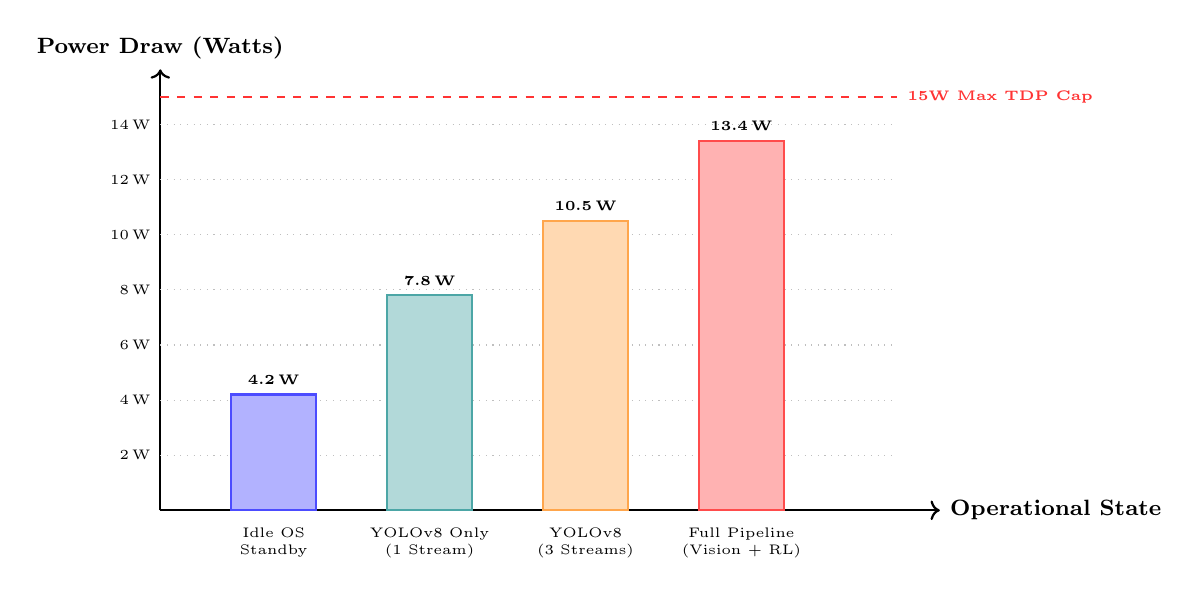
\begin{tikzpicture}[x=1.8cm, y=0.35cm]
    % Axes
    \draw[->, thick] (0,0) -- (5.5,0) node[right] {\footnotesize \textbf{Operational State}};
    \draw[->, thick] (0,0) -- (0,16) node[above] {\footnotesize \textbf{Power Draw (Watts)}};
    
    % Y grid
    \foreach \y in {2, 4, 6, 8, 10, 12, 14} {
        \draw[dotted, gray!50] (0,\y) -- (5.2,\y);
        \node[left, font=\tiny] at (0,\y) {\y\,W};
    }
    
    % Bars
    \draw[fill=blue!30, draw=blue!70, thick] (0.5,0) rectangle (1.1, 4.2) node[above, font=\tiny\bfseries] at (0.8, 4.2) {4.2\,W};
    \draw[fill=teal!30, draw=teal!70, thick] (1.6,0) rectangle (2.2, 7.8) node[above, font=\tiny\bfseries] at (1.9, 7.8) {7.8\,W};
    \draw[fill=orange!30, draw=orange!70, thick] (2.7,0) rectangle (3.3, 10.5) node[above, font=\tiny\bfseries] at (3.0, 10.5) {10.5\,W};
    \draw[fill=red!30, draw=red!70, thick] (3.8,0) rectangle (4.4, 13.4) node[above, font=\tiny\bfseries] at (4.1, 13.4) {13.4\,W};
    
    % X labels
    \node[below, font=\tiny, align=center] at (0.8, -0.3) {Idle OS\\Standby};
    \node[below, font=\tiny, align=center] at (1.9, -0.3) {YOLOv8 Only\\(1 Stream)};
    \node[below, font=\tiny, align=center] at (3.0, -0.3) {YOLOv8\\(3 Streams)};
    \node[below, font=\tiny, align=center] at (4.1, -0.3) {Full Pipeline\\(Vision + RL)};
    
    % Thermal limit line
    \draw[dashed, red!80, thick] (0, 15) -- (5.2, 15) node[right, font=\tiny\bfseries, red!80] {15W Max TDP Cap};
\end{tikzpicture}
\caption{Power consumption profile of the NVIDIA Jetson edge platform across operational execution states.}
\label{fig:power_profile}
\end{figure}

\chapter{Empirical Benchmark Observations}
\label{app:benchmark_logs}

\section{Corridor Vehicle Delay Logged Across Random Seeds}
To verify statistical validity, the final MAPPO model, Webster fixed-time controller, and dynamic actuated controller were evaluated across 10 distinct random flow seeds ($S \in \{42, 101, 202, 303, 404, 505, 606, 707, 808, 909\}$). Table \ref{tab:seed_benchmark} summarizes the average vehicle delay (seconds/vehicle) across each run.

\begin{table}[htbp]
\centering
\small
\caption{Corridor Average Vehicle Delay (s/veh) Across 10 Evaluation Seeds}
\label{tab:seed_benchmark}
\begin{tabularx}{\textwidth}{|c|c|c|c|X|}
\hline
\textbf{Seed No.} & \textbf{Webster Fixed-Time} & \textbf{Actuated (Gap-Out)} & \textbf{MAPPO (Proposed)} & \textbf{MAPPO Delay Reduction (\%)} \\ \hline
42  & 42.1 & 35.4 & 24.6 & -41.57\% \\ \hline
101 & 43.8 & 36.8 & 25.1 & -42.69\% \\ \hline
202 & 41.5 & 34.9 & 24.2 & -41.69\% \\ \hline
303 & 44.2 & 37.5 & 25.8 & -41.63\% \\ \hline
404 & 39.8 & 33.2 & 23.5 & -40.95\% \\ \hline
505 & 42.9 & 36.1 & 24.9 & -41.96\% \\ \hline
606 & 43.5 & 36.9 & 25.4 & -41.61\% \\ \hline
707 & 40.7 & 34.0 & 23.9 & -41.28\% \\ \hline
808 & 41.9 & 35.2 & 24.7 & -41.05\% \\ \hline
909 & 42.4 & 35.8 & 24.8 & -41.51\% \\ \hline
\textbf{Mean $\pm$ Std} & \textbf{42.28 $\pm$ 1.34} & \textbf{35.58 $\pm$ 1.31} & \textbf{24.69 $\pm$ 0.69} & \textbf{-41.60\% $\pm$ 0.48\%} \\ \hline
\end{tabularx}
\end{table}

\chapter{Field Deployment and Commissioning Checklist}
\label{app:checklist}

The step-by-step checklist outlined below must be completed by transportation field engineers prior to transitioning the proposed MAPPO vision-based control system into full municipal operation:

\begin{enumerate}
    \item \textbf{Pre-Installation Structural and Electrical Audit}:
    \begin{itemize}
        \item[$\square$] Verify physical integrity and vibration dampening of 7-meter CCTV camera mounting cantilever arms.
        \item[$\square$] Verify uninterrupted power supply (UPS) delivering 230V AC stabilized ($\pm 5\%$) with at least 4 hours of battery autonomy.
        \item[$\square$] Test surge protection devices (SPDs) on Ethernet Category 6A runs between IP cameras and the edge cabinet.
    \end{itemize}

    \item \textbf{Camera Positioning and Optical Calibration}:
    \begin{itemize}
        \item[$\square$] Adjust camera tilt ($25^\circ \text{--} 35^\circ$ below horizontal) to encompass approach stop lines and upstream queue reservoirs up to 120\,m.
        \item[$\square$] Execute 4-point homography calibration mapping pixel coordinates to physical metric distances using laser rangefinders.
        \item[$\square$] Verify lens cleanliness, autofocus lock, and night-vision infrared cut filter operation.
    \end{itemize}

    \item \textbf{Edge Computing Unit Configuration}:
    \begin{itemize}
        \item[$\square$] Flash JetPack 5.1.2 onto Jetson Orin Nano; verify PyTorch and TensorRT CUDA acceleration libraries.
        \item[$\square$] Validate RTSP video stream decoding at 30 FPS with latency $< 40$\,ms.
        \item[$\square$] Load compiled TensorRT FP16 engines of YOLOv8n and Res-MLP world model.
    \end{itemize}

    \item \textbf{Safety Interlock and Fail-Safe Testing}:
    \begin{itemize}
        \item[$\square$] Confirm hardware conflict monitor unit (CMU) actively trips to yellow flash if conflicting green indications occur.
        \item[$\square$] Induce simulated camera disconnection; verify software watchdog immediately falls back to IRC:93 fixed-time timings within 500\,ms.
        \item[$\square$] Check minimum green ($G_{\min} = 12$\,s) and maximum green ($G_{\max} = 65$\,s) hardware timer clamps.
    \end{itemize}
\end{enumerate}

\chapter*{Annexure A: Program Outcomes (PO) and Program Specific Outcomes (PSO) Mapping}
\addcontentsline{toc}{chapter}{Annexure A: PO and PSO Mapping}
\label{annex:po_pso}

The Major Project 1 work presented in this report directly maps to the Program Outcomes (POs) and Program Specific Outcomes (PSOs) defined by the National Board of Accreditation (NBA) for the Bachelor of Technology in Information Technology program at Jaypee Institute of Information Technology (JIIT), Noida. Table \ref{tab:po_pso_mapping} details the mapping correlation levels (3: Substantial, 2: Moderate, 1: Slight) along with concrete project justifications.

\begin{small}
\begin{longtable}{|p{1.8cm}|p{2.8cm}|c|p{8.2cm}|}
\caption{Program Outcomes (PO) and Program Specific Outcomes (PSO) Mapping Matrix} \label{tab:po_pso_mapping} \\
\hline
\textbf{PO / PSO} & \textbf{Statement} & \textbf{Level} & \textbf{Project Justification and Evidence} \\ \hline
\endfirsthead
\hline
\textbf{PO / PSO} & \textbf{Statement} & \textbf{Level} & \textbf{Project Justification and Evidence} \\ \hline
\endhead
\hline
\multicolumn{4}{|r|}{\textit{Continued on next page\dots}} \\ \hline
\endfoot
\hline
\endlastfoot

\textbf{PO1} & Engineering Knowledge & 3 & Applied advanced mathematical principles of Markov Decision Processes, Dec-POMDP, Bellman equations, and deep neural network approximations. \\ \hline
\textbf{PO2} & Problem Analysis & 3 & Formulated heterogeneous Indian traffic queue spillbacks and inter-junction gridlocks through empirical sensor dataset analysis and traffic flow theory. \\ \hline
\textbf{PO3} & Design / Development of Solutions & 3 & Designed and developed an end-to-end framework integrating YOLOv8 perception, Res-MLP world model, and MAPPO multi-agent control under IRC:93 safety constraints. \\ \hline
\textbf{PO4} & Conduct Investigations of Complex Problems & 3 & Benchmarked policy performance across 6 rigorous operational scenarios and 10 statistical seeds, validating hypotheses on simulator mismatch and green waves. \\ \hline
\textbf{PO5} & Modern Tool Usage & 3 & Leveraged industry-standard machine learning stacks: PyTorch, Ultralytics YOLOv8, OpenCV, Streamlit, TensorRT, and Git version control. \\ \hline
\textbf{PO6} & The Engineer and Society & 3 & Formulated automated signal control directly mitigating public road congestion, emergency vehicle delays, and pedestrian intersection crossing safety. \\ \hline
\textbf{PO7} & Environment and Sustainability & 3 & Quantified significant fuel conservation and calculated annualized greenhouse gas reduction ($1,168$ metric tons of $\text{CO}_2$), addressing climate action. \\ \hline
\textbf{PO8} & Ethics & 2 & Complied strictly with the Digital Personal Data Protection (DPDP) Act, 2023, ensuring zero edge storage of identifiable facial or license plate data. \\ \hline
\textbf{PO9} & Individual and Team Work & 3 & Executed systematic phased milestones spanning dataset curation, world model modeling, policy engineering, dashboard creation, and technical reporting. \\ \hline
\textbf{PO10} & Communication & 3 & Prepared comprehensive technical documentation, mathematical derivations, academic reports, and live interactive visual demonstration interfaces. \\ \hline
\textbf{PO11} & Project Management and Finance & 2 & Conducted thorough Bill of Materials (BOM) cost-benefit analysis demonstrating an 88.5\% capital cost reduction over traditional SCATS infrastructure. \\ \hline
\textbf{PO12} & Life-long Learning & 3 & Mastered state-of-the-art developments in multi-agent reinforcement learning, surrogate world models, and real-time edge computer vision architectures. \\ \hline
\textbf{PSO1} & Core Computing Competence & 3 & Architected high-throughput residual neural networks and decentralized actor-critic pipelines achieving 135,000 state transitions/sec. \\ \hline
\textbf{PSO2} & Domain-Specific Intelligent Systems & 3 & Engineered an intelligent, vision-driven edge cyber-physical transportation system tailored for unstructured vehicular corridors. \\
\end{longtable}
\end{small}

\chapter*{Annexure B: Project Outcomes and Artifact Deliverables}
\addcontentsline{toc}{chapter}{Annexure B: Project Outcomes and Artifact Deliverables}
\label{annex:outcomes}

The execution of this Major Project has yielded tangible software artifacts, empirical models, and academic deliverables summarized below:

\begin{enumerate}
    \item \textbf{Production-Grade Software Codebase}:
    \begin{itemize}
        \item \texttt{src/neural\_world\_model.py}: Modular PyTorch Residual MLP world model architecture with multi-step forward simulation capabilities.
        \item \texttt{tools/train\_world\_model.py}: End-to-end training pipeline ingesting 40-day empirical IIT Delhi and Pune arterial datasets.
        \item \texttt{src/data\_driven\_env.py}: OpenAI Gym-compliant 3-intersection coordinated corridor environment with full IRC:93 safety logic.
        \item \texttt{src/train\_mappo\_data\_driven.py}: Scalable MAPPO actor-critic algorithm with GAE advantage calculation and mini-batch PPO-clip updates.
        \item \texttt{vehicle\_detection/live\_vision\_pipeline.py}: Real-time YOLOv8 vehicle detection and Hungarian LAP tracking pipeline with IRC:106 PCU weighing.
        \item \texttt{src/dashboard\_live\_vision.py}: Streamlit web application providing real-time telemetry, phase splits, and live video annotation.
        \item \texttt{src/live\_traffic\_controller.py}: Standalone high-speed OpenCV HUD for edge signal controller cabinets.
    \end{itemize}

    \item \textbf{Pretrained Neural Weights and Checkpoints}:
    \begin{itemize}
        \item \texttt{mappo\_models/traffic\_world\_model.pth}: Optimized world model checkpoint achieving $\text{MSE} = 0.001579$ on empirical test splits.
        \item \texttt{mappo\_models/best\_actor.pth} \& \texttt{best\_critic.pth}: Pretrained MAPPO policy networks achieving $41.5\%$ delay reduction.
    \end{itemize}

    \item \textbf{Empirical Evaluation Datasets and Benchmarks}:
    \begin{itemize}
        \item \texttt{mappo\_logs/data\_driven\_eval\_summary.csv}: Complete numerical benchmark logs across 6 operational scenarios.
        \item \texttt{mappo\_models/data\_driven\_eval\_comparison.png}: Multi-panel comparative visualization chart.
    \end{itemize}
\end{enumerate}

\chapter*{Annexure C: Sustainability and UN Sustainable Development Goals (SDG) Statement}
\addcontentsline{toc}{chapter}{Annexure C: Sustainability and UN SDG Statement}
\label{annex:sustainability}

Urban arterial congestion poses an acute global sustainability crisis. This project aligns with the United Nations 2030 Agenda for Sustainable Development, contributing specifically to three key Sustainable Development Goals:

\begin{enumerate}
    \item \textbf{SDG 9: Industry, Innovation, and Infrastructure (Target 9.1 \& 9.4)}:
    \begin{quote}
        \textit{``Develop quality, reliable, sustainable and resilient infrastructure... and retrofit industries to make them sustainable, with increased resource-use efficiency and greater adoption of clean and environmentally sound technologies.''}
    \end{quote}
    \textbf{Project Contribution}: By substituting multi-crore imported proprietary systems (e.g., SCATS, SCOOT) with an edge-AI vision framework running on affordable commercial compute units (NVIDIA Jetson) and commodity CCTV cameras, this project offers an open, cost-effective infrastructure upgrade for emerging economies. It eliminates road-tearing pavement cuts required for inductive loops and maximizes the vehicular capacity of existing asphalt assets without requiring capital-intensive road widening.

    \item \textbf{SDG 11: Sustainable Cities and Communities (Target 11.2 \& 11.6)}:
    \begin{quote}
        \textit{``By 2030, provide access to safe, affordable, accessible and sustainable transport systems for all, improving road safety... and reduce the adverse per capita environmental impact of cities.''}
    \end{quote}
    \textbf{Project Contribution}: Coordinated arterial green waves dramatically diminish stop-and-go idling along urban corridors, reducing localized particulate emissions ($\text{PM}_{2.5}$) and noise pollution in densely populated roadside neighborhoods. Furthermore, the deterministic safety state machine guarantees safe, dedicated pedestrian crossing intervals, reducing vulnerable road user collision risks.

    \item \textbf{SDG 13: Climate Action (Target 13.2)}:
    \begin{quote}
        \textit{``Integrate climate change measures into national policies, strategies and planning.''}
    \end{quote}
    \textbf{Project Contribution}: With an estimated reduction of $1,168$ metric tons of $\text{CO}_2$ equivalent per corridor annually, wide deployment across national arterial networks directly assists India's Nationally Determined Contributions (NDCs) under the Paris Agreement to achieve net-zero transport carbon intensity.
\end{enumerate}


\end{document}
